% !TEX root = approx8.tex

\section{Nearby Approximability}\label{sec:nearby}
 
 The aim of this section is to prove an approximability result, Theorem \ref{thm:nearby},  which is formulated in \S \ref{subsec:state}. In the last subsection, \S\ref{subsec:nearby-TPC},  the first point  of Theorem  \ref{thmmain1} is  seen to easily follow  from Theorem \ref{thm:nearby}. 

 \subsection{Setting}\label{subsec:back} We start by providing some necessary notation and background.
 
 Let $(N^{n},\mathtt{g})$ be a closed $n$-manifold with Riemannian metric $\mathtt{g}$. 
 We denote by $D_{r}^{\ast}N$ the closed $r$-disk cotangent bundle of $N$, with respect to  the  metric corresponding to $\mathtt{g}$ (under the identification $T^{\ast}N\cong TN$, induced by $\mathtt{g}$) $$D_{r}^{\ast}(N)\subset T^{\ast}N~.~$$
 We endow $T^{\ast}N$ with the canonical symplectic form
 $\omega=d\lambda$ with $\lambda$ the Liouville $1$-form on $T{^\ast}N$.
 
 We consider the class $\lagex(D^{\ast}_{r}N)$ of all closed, {\em exact} Lagrangian submanifolds in the interior of $D_{r}^{\ast}N$, see \S\ref{sb:fuk-ex}. For $r=1$, we simplify the notation by omitting the subscript $r$. There are filtered Fukaya categories with objects the elements in $\lagex(D^{\ast}_{r}N)$ denoted by $\fuk(\lagex(D^{\ast}_{r}N); p)$ where $p\in\mathcal{P}$ is a choice of perturbations, as described in Chapter \ref{ch:ffuk}.   To simplify the various constructions below we denote $\mathcal{A}_{p}(r)=\fuk(\lagex(D^{\ast}_{r}N); p)$. We  omit $p$ from the notation, when this parameter is fixed and no confusion is possible and in case $r=1$ we write $\mathcal{A}_{p}$ instead of $\mathcal{A}_{p}(r)$. 
 
The considerations below are independent of $r$ and thus we fix $r=1$.
 The Yoneda functor embeds $\mathcal{A}_{p}$ inside the category 
 of filtered $A_{\infty}$ modules, $
 F\md_{\mathcal{A}_{p}}$,
 $$\mathcal{Y}_{p}: \mathcal{A}_{p}\hookrightarrow F\md_{\mathcal{A}_{p}}~.~$$
 
 For a point $x\in N$, let $\overline{F}_{x}$ be the cotangent fiber through $x$,
 $$\overline{F}_{x}=\pi^{-1}(x)$$ where  $\pi : T^{\ast}N\to N$  is the projection of the cotangent bundle. Such a fiber also admits markings and we denote by $F_{x}= (\overline{F}_{x}, h_{F_{x}}, \theta_{F_{x}})$ a marked fiber, with underlying Lagrangian submanifold $\overline{F}_{x}$ ($h_{F_{x}}$ 
 is a constant function in this case). Each $F_{x}$ defines a filtered $A_{\infty}$-module still denoted  
 $$F_{x}\in F\md_{\mathcal{A}_{p}}~.~$$  
 For this it is necessary to define the perturbations required for
 defining $\mu_{d}$ operations involving tuples of closed Lagrangians and one copy of $\overline{F}_{x}$. 
 Denoting marked Lagrangians and the  associated Yoneda modules  by the same symbols simplifies notation and it is generally non-problematic, however it is important to keep track of the precise context, namely of the underlying $A_{\infty}$-category.
 With these conventions, we have $F_{x}(L)=CF(L,F_{x}; p)$ as filtered chain complexes.  
 
\

We denote by ${\mathcal{A}^{F}_{p}}$ the filtered full sub-category of $F\md_{\mathcal{A}_{r}}$ that contains the image  of $\mathcal{Y}_{p}$, and all the modules ${F}_{x}$, $x\in N$ (with all possible markings on the fibers $\overline{F}_{x}$). As before,
in case we want to render explicit both the perturbation parameter $p$ and the radius of the 
disk bundle $D^{\ast}_{r}N$ we write $\mathcal{A}^{F}_{p}(r)$. 

\

The next step is to complete each category ${\mathcal{A}^{F}_{p}}$ with respect to mapping cones over morphisms with filtration level $\leq 0$ and quasi-isomorphisms of filtration level $\leq 0$ and denote the result by $[\mathcal{A}^{F}_{p}]^{\Delta}$. Finally, we let 
$\msc_{p}$ be the associated TPC, $\msc_{p}=PH([\mathcal{A}^{F}_{p}]^{\Delta})$. The categories 
$\mathcal{A}^{F}_{p}$ fit into a system of filtered categories for varying $p$.  Thus we have functors $\mathcal{H}_{p,q}:\mathcal{A}^{F}_{p}\to \mathcal{A}^{F}_{q}$ defined using the 
push-forward construction of filtered modules. More specifically,
recall that for $p \preceq q$ we have a continuation functor
$\mathcal{H}^{\text{cont}}_{p,q} : \mathcal{A}_p \longrightarrow
\mathcal{A}_q$. The functor $\mathcal{H}_{p,q}$ is defined as
$\mathcal{H}_{p,q} := (\mathcal{H}^{\text{cont}}_{p,q})_*$, the
induced push-forward of modules. The functors $\mathcal{H}^{\text{cont}}_{p,q}$ preserve filtration whenever $p\preceq q$. We also have functors $\mathcal{H}^{\text{cont}}_{q,p}$, however these are $A_{\infty}$-functors with a possibly non-vanishing linear deviation  (see \S\ref{sb:sys-ainfty}).

Summing up,  we obtain comparison functors, still denoted  
$\mathcal{H}_{p,q}: \msc_{p}\to \msc_{q}$. The categories $[\mathcal{A}^{F}_{p}]^{\Delta}$ are pre-triangulated and as a result the system  $\widehat{\msc}(D^{\ast}N) =(\msc_{p}, \mathcal{H}_{p,q})$ forms a system of TPCs with increasing accuracy in the sense of \S\ref{s:sys-tpc}.  


 \subsection{The main statement, and the idea of the proof}\label{subsec:state}

Using the system $\widehat{\msc}(D^{\ast}(N))$ of TPCs we can now formulate the main result of the section.

\

To proceed, recall the equivalence relation in \S\ref{sb:sys-inv} defined on 
$$\Ob^{\text{tot}}(\widehat{\msc}(D^{\ast}N)) := \coprod_{p\in \mathcal{P}} \Ob(\msc_p)~.~$$
 The set of associated equivalence classes
is denoted by $\widetilde{\Ob}(\widehat{\msc}(D^{\ast}N))$. 
All exact, marked, Lagrangians $L\in \mathcal{L}ag^{(ex)}(D^{\ast}N)$ correspond to well-defined equivalence classes in $\widetilde{\Ob}(\widehat{\msc}(D^{\ast}N))$  because $\mathcal{H}_{p,q}$ takes Yoneda modules to modules $0$-equivalent to Yoneda modules whenever $p\preceq q$. We denote
by $\mathcal{L}(D^{\ast}N)\subset \widetilde{\Ob}(\widehat{\msc}(D^{\ast}N))$ the set of equivalence classes of all such, closed, exact, marked $L$'s. We formulate a similar property for a family of marked fibers $\F=\{F_{x_{1}},\ldots, F_{x_{i}},\ldots\}$ of $D^{\ast}N$. We say that the family
$\F$ satisfies property ($\ast$) if:

\begin{itemize}
\item[($\ast$)]
 {\it for all $p \preceq q$, for every marked fiber
$F_{x} \in \F$ we have $\mathcal{H}_{p,q}(F_{x}) \cong_0 F_{x}$, where the $F_{x}$ on the right-hand side of $\cong_0$ stands for the  module corresponding to 
$F_{x}$ in $\Ob(\msc_{q})$.} 
\end{itemize}
If this property is satisfied by the family $\F$, then  each marked fiber $F_{x}\in \F$ corresponds to a well-defined equivalence class $\mathscr{F}_{x}\in\widetilde{\Ob}(\widehat{\msc}(D^{\ast}N))$. 


\begin{thm}\label{thm:nearby}
Fix $\varepsilon>0$. It is possible to construct the system $\widehat{\msc}(D^{\ast}(N))$ such that  there is a finite family of marked fibers $\F_{\varepsilon}=\{F_{x_{1}}, \ldots, F_{x_{l}}\}$ that satisfies property {\rm ($\ast$)} and, moreover, the set $\mathcal{L}(D^{\ast}N)$ is $\varepsilon$-approximable in the sense of Definition \ref{d:approx-sys} by $\{\mathscr{F}_{x_{1}},\ldots, \mathscr{F}_{x_{l}}\}$.
\end{thm}


In other words, for some $\beta = \beta(\varepsilon) >0$ we have that for each $L\in\mathcal{L}ag^{(ex)}(D^{\ast}N)$ and each $p$ with 
$\nu(p)\leq \beta$ there is an iterated cone $C$ inside $\msc_{p}$ constructed by using  the marked fibers $(\overline{F}_{x_{i}},  \alpha_{x_{i}})$, for some constants $\alpha_{x_{i}}\in \R$ (and some choice of grading),  such that $C$ is at interleaving  distance at most $\varepsilon$ from $L$ in $\msc_{p}$.  Of course, we identify here a Lagrangian $L$ with its corresponding Yoneda module. Moreover, fitting the categories $\msc_{p}$ in the system $\widehat{\msc}(D^{\ast}N)$
renders the relevant construction independent of the choice of $p$, as long as $\nu(p)$ is small enough.

\

We will see in \S\ref{subsec:nearby-TPC} that this result immediately implies approximability in the sense of Definition \ref{def:TPC-approx} and thus  point i of Theorem \ref{thmmain1} is established.

\begin{rem}\label{rem:dep_on_e} The dependence of the statement 
on $\varepsilon$ is subtle. It is possible to construct the system $\widehat{\msc}(D^{\ast}N)$ such that each category $\msc_{p}$ is independent of $\varepsilon$ (for $\nu(p)$ small) and  all the disk bundle fibers, and in particular  all the elements of  $\F_{\varepsilon}$, for all $\varepsilon$,  are represented as modules in $\msc_{p}$. However, the system
$\widehat{\msc}(D^{\ast}N)$ also depends on the functors $\mathcal{H}_{p,q}$ and these functors need to be so that they satisfy property ($\ast$) relative to the family of fibers $\F_{\varepsilon}$. In our argument, this property follows from a geometric construction that is the central part of the proof and that requires a fixed $\varepsilon$ as starting point. As a result, when $\varepsilon$ changes, apriori, the system $\widehat{\msc}(D^{\ast}N)$ changes too, along with the family
$\F_{\varepsilon}$ whose number of elements increases when 
$\varepsilon$ tends to $0$.  See also Remark \ref{rem:compare_data}.
\end{rem}

\

%\begin{rem} 
% Categorical metric-approximability has another meaningful formulation in the context of triangulated persistence categories. 
% One feature of a TPC $\mathcal{\C}$ is that it is endowed with a class of weighted triangles, with non-negative weights, satisfying weighted analogues of the axioms of exact triangles in a triangulated category. As a result, the set $\mathcal{O}bj (\mathcal{\C})$ is endowed with a family of pseudo-metrics $d^{\mathcal{F}}$ for each  family $\mathcal{F}\subset \mathcal{O}bj (\mathcal{\C})$. These so-called 
% fragmentation pseudo-metrics are infimizing the total weight of triangles needed to  construct one object $A$ from another  $A'$ by iterated triangles of the 
% form:
% $$F_{i}\to A_{i}\to A_{i+1}\to TF_{i}$$ with $F_{i}\in \mathcal{F}^{\Sigma}$  except for one index $j$ for which $F_{j}=T^{-1}A'$, $A_{0}=0$ and 
% with the last term $A_{k}=A$ (this is then symmetrized).
% The simplest and largest distance $d^{\emptyset}$ 
% is defined for $\mathcal{F}=\emptyset$. It coincides 
% with the TPC version of the interleaving distance $d_{int}$ mentioned before.  This distance is natural but often infinite. On the other hand, an inclusion $\mathcal{F}\subset \mathcal{F}'$ implies $d^{\mathcal{F}}\geq 
% d^{\mathcal{F}'}$ so by enlarging the family $\mathcal{F}$ one can expect the associated pseudo-metrics to decrease. 
% 
%It is immediate to see that  $\mathcal{S}\subset \mathcal{O}b(\C)$ is categorically approximable iff for any $\varepsilon$ there 
% is a finite family $\mathcal{F}_{\varepsilon}$ such that $$Diam_{d^{\mathcal{F}_{\varepsilon}}}(\mathcal{S}) \leq \varepsilon~.~$$
% 
% \end{rem}

\subsubsection{Outline of the proof of Theorem \ref{thm:nearby}.} 

The  proof proceeds roughly as follows.  We first establish the existence
of some special Morse functions that have small variation and large gradient away from their critical points. More precisely, denote by $B_{\eta}(x)$ the disk in $N$ (with respect to the metric $g$) of radius $\eta$ and center at $x\in N$.  
For any values $K, \delta >0$ and sufficiently small $\eta >0$ there
exists a Morse function $f:N\to [0, K]$ such that $||d f_{x}||\geq \delta$ for all points $x\in N\backslash (\cup_{z\in Crit(f)} B_{\eta}(z))$.  We then consider a Lefschetz 
fibration structure on $T^{\ast}N$, $p:T^{\ast}N\to \mathbb{C}$, 
as constructed by  Giroux \cite{Gir:Lef-cot}, such that the real part of the projection $p$ coincides with a Morse function
 $f$ with the properties above, with $1>\delta>0$ fixed and $K$ small. We then use a method introduced in \cite{Bi-Co:lefcob-pub} to surger each exact Lagrangian with a certain number of (compactifications) of the fibers through $Crit(f)$ and  use a Hamiltonian isotopy to push the result away from $D^{\ast}N$.  This part of the construction takes place in the total space $E$ of a modified Lefschetz fibration that is constructed along the approach in \cite{Bi-Co:lefcob-pub}.  Algebraically,
this process  expresses the Lagrangian as an iterated cone of fibers and an $s$-acyclic term, where $s$ is at most equal to the Hofer energy needed to generate the previous Hamiltonian displacement. The key point is to control this energy. This is where  the fact that $K$ is small (and $\delta$ is relatively big) comes into play:  through some precise estimates that appear in Giroux's construction we show that this energy  can be related to the area of a certain planar region corresponding to the projection on $\mathbb{C}$ of $D^{\ast}N$, and, as a result, it is bounded uniformly, independently of $L$, by a constant times $K$.

The  steps required for the proof of Theorem \ref{thm:nearby} are each contained in a subsection below, as follows.  In \S\ref{subsec:Morse} we outline the construction of the special Morse functions with small variation but big differential away from the critical points. This is a soft result, but not completely trivial. In \S\ref{subsec:Giroux} we review the main ingredients in Giroux's construction. Next, in \S\ref{subsec:Lef-Dehn} we
recall the approach from \cite{Bi-Co:lefcob-pub} and adjust it to Giroux's set-up. Most of the proof -  in \S\ref{subsec:Morse}, \S\ref{subsec:Giroux}, \S\ref{subsec:Lef-Dehn} and \S\ref{subsec:finish-proof} up to \S\ref{subsubsec:back_to_alg} -  is entirely geometric and serves to establish the statement in Proposition \ref{lem:disj_fibers} which, essentially,  claims that:

{\em  Given $\varepsilon >0$ there exists a Lefschetz fibration $p:E\to \mathbb{C}$ that contains $D^{\ast}N$ and such that there are exact Lagrangian spheres $\hat{S}_{1},\ldots, \hat{S}_{l}$ in $E$, each of them intersecting $D^{\ast}N$ along a (different) fiber of $D^{\ast}N$, with the property that, for any exact, closed Lagrangian $L\subset D^{\ast}N$, the iterated Dehn twist $\tau_{\hat{S}_{l}}(\tau_{\hat{S}_{l-1}} (\ldots \tau_{\hat{S}_{1}}(L)).. )$ can be disjoined from $D^{\ast}N$ by a Hamiltonian diffeomorphism of Hofer norm at most $\varepsilon$.}

The last part 
of the proof of Theorem \ref{thm:nearby}, in \S\ref{subsubsec:back_to_alg}, translates this geometric result in an appropriate system  $\widehat{\msc}(D^{\ast}N)$. 

\subsection{Special Morse functions }\label{subsec:Morse}
\begin{prop}\label{prop:Morse}
Let $(N^{n},\mathtt{g})$ be a smooth, closed riemannian manifold . For any $K>0$, $1>\delta >0$ and  
$\eta>0$ there exists a Morse function $\varphi=\varphi_{N, K,\delta}:N\to [0,K]$ with the property
that $ ||d\varphi(x)||\geq\delta$ for all $x\in N\backslash (\cup_{z\in Crit(\varphi_{N, K,\delta})} B_{\eta_{z}}(z))$, where $0<\eta_{z}\leq \eta$, $\forall z\in Crit(\varphi_{N, K,\delta})$.
\end{prop} 
Notice that we assume here that the radius $\eta_{z}$ of the ball $B_{\eta_{z}}(z)$ around 
the critical points $z$ of $f$ depends on the critical point.  We also assume that all these balls $B_{\eta_{z}}$ are pairwise disjoint. 
\begin{proof}  To start the proof we fix a Morse function $f_{0}:N\to \R$
as well as some small quantity $\alpha>0$. We assume that the function $f_{0}$
and the metric  $\mathtt{g}$ are standard inside $B_{\alpha}(z)$ in the neighbourhoods $B_{\alpha}(z)$ for each $z\in Crit(f_{0})$. These two conditions
are not essential for the argument, they just simplify some of the calculations
in the proof. With these assumptions,  the gradient (calculated with respect to $\texttt{g}$) 
$\nabla f_{0}$ is standard, of the form $k(\ldots, \pm x_{i}\partial/\partial x_{i},\ldots)$ with respect to coordinates $(x_{1},\ldots, x_{i},\ldots, x_{n})$
inside each $B_{\alpha}(z)$; $k$ is a constant that depends on $z$. We also assume that $f_{0}$ has $m$ critical points $z_{0},\ldots, z_{m-1}$ and $f_{0}(z_{j})=jB$ for some positive constant $B$.
After possibly
multiplying $f_{0}$ with a large positive constant we may assume that $||df_{0}||\geq \delta$ outside the union of all the balls $B_{\alpha}(z)$.  We denote by $V=(m-1)B$ the maximal value of $f_{0}$.  We let $U_{z}(\mu)=f_{0}^{-1}([f_{0}(z)-\mu, f_{0}(z)+\mu])$ and 
$U'_{z}(\mu)=f_{0}^{-1}([f_{0}(z)-\mu/2, f_{0}(z)+\mu/2])$ and assume that $B_{\alpha}(z)$
is contained in $U'_{z}(\mu)$. We fix $\mu>0$ so  that all
these sets $U_{z}(\mu)$ are pairwise disjoint and to simplify notation below
we denote $U_{z}=U_{z}(\mu)$, $U'_{z}=U'_{z}(\mu)$.

We will modify $f_{0}$ with two aims:  diminish the variation $V$ and decrease the size of the neighbourhoods $B_{z}(\alpha)$, in both cases as much as needed. Of course, the price to pay is that we will add many new additional critical points
to those of $f_{0}$. The argument uses induction on the dimension of $N$. Thus, we assume the Proposition established for all manifolds of dimension at most $n-1$ (it is an easy exercise to prove the result in dimension $1$).

The modifications of the function $f_{0}$ are of two types. 

The first is a change inside a small
neighbourhood of each critical point $z$ of $f_{0}$. We will later refer to this step as ``shrinking''. To simplify notation we fix such a critical
point and its critical value $v=f(z)$. We consider $\eta <\alpha/2$ and a ball $B_{\eta}(z)$ as well as the larger ball $B_{2\eta}$.
We then consider a diffeomorphism $\psi_{z}:U'_{z}\to U_{z}$ with the following properties:
\begin{itemize}
\item[-] $\psi_{z}(f_{0}^{-1}(v\pm\mu/2))=f_{0}^{-1}(v\pm\mu)$.
\item[-] $\psi_{z}$ preserves  $f^{-1}(v)$.
\item[-] $\psi_{z}$ maps  $B_{2\eta}(z)$ to $B_{\alpha}(z)$ while keeping $z$ fixed and on $B_{\eta}(z)$ is acts by $x \to rx$ where 
$r>1$ is given by $r^{2} =\frac{\delta}{\eta k}$ (this obviously assumes $\eta$ small enough, see also the next point).
\item[-] we assume $\eta$ small enough such that that $2r\eta = 2\sqrt{\frac{\delta\eta}{k}} <\alpha$.
\item[-]  $\psi_{z}$ 
transports $f_{0}^{-1}(v-\mu/2)$ along the flow of $-\nabla f_{0}$, mapping it to
$f_{0}^{-1}(v-\mu)$, and it transports 
 $f_{0}^{-1}(v+\mu/2)$ along the flow of $+\nabla f_{0}$, sending it to $f_{0}^{-1}(v+\mu)$.
\end{itemize}
It is easy to construct such a diffeomorphism, see Figure \ref{fig:expand}. 
\begin{figure}
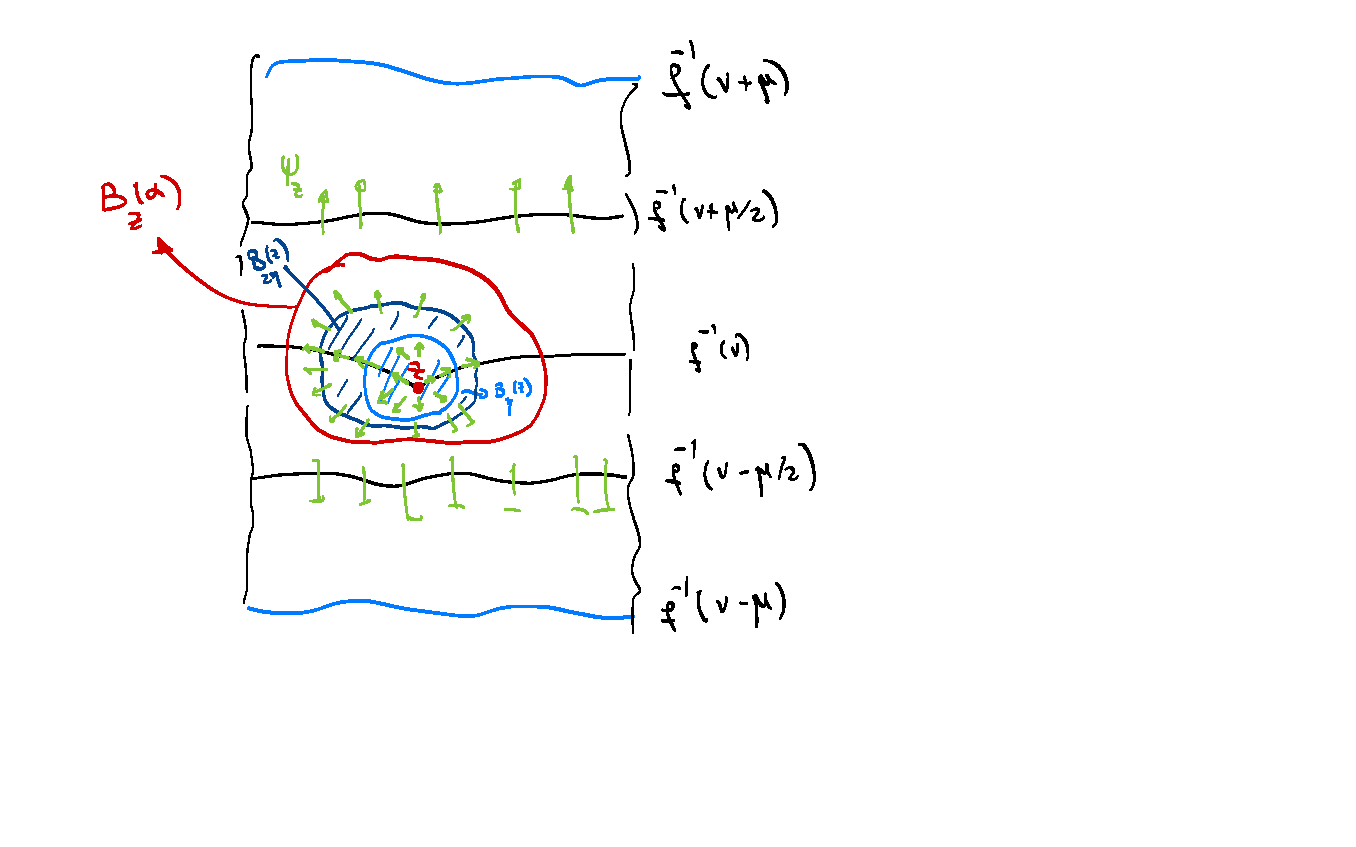
\includegraphics[scale=0.9]{expand.pdf}
  \centering
  \caption{The diffeomorphism $\psi_{z}$.} \label{fig:expand}
\end{figure}



We now define
a new function $f_{1}$ as follows: on the set $U'_{z}$ it is given by $f_{0}\circ \psi_{z}$; on the set $f_{0}^{-1}(-\infty, v-\mu/2]$ it is equal to $f_{0}-\mu/2$; on the set $f_{0}^{-1}[v+\mu/2,\infty)$ it is equal to $f_{0}+\mu/2$.
Notice that this function is continuous, of total variation $V+\mu$,
but not smooth along $f_{0}^{-1}(v\pm \mu/2)$. However,
it can be smoothed along these two hypersurfaces, and by this smoothing - still denoted $f_{1}$ -  does not add any new critical points and  $||df_{1}(x)||\geq \delta$ for all points $x$ outside $B_{2\eta}(z)$. 

The total variation of the  perturbed function $f_{1}$ is smaller than $V+2\mu$, by taking the smoothing sufficiently small. 
We now discuss the role of two of the  properties of $\psi_{z}$. The role of the third  property is to ensure that $||df_{1}(x)||\leq \delta$ for $x\in B_{\eta}(z)$ (this property will be important for us later in the proof of the proposition). 
This is easily seen as $||\nabla f_{0}(x)||= k ||x||$ inside $B_{\alpha}(z)$
and thus $||\nabla f_{1}(x)||=r k ||r x||= r^{2}k ||x||=\delta\frac{||x||}{\eta}$ for $x\in B_{\eta}(z)$. The role of the fourth property is to allow for
enough ``room'' so that $||df_{1}(x)||\geq \delta $ for the points $x\in B_{2\eta}(z)\backslash B_{\eta}(z)$.

We apply this procedure for each critical point of $f_{0}$ and we call the resulting function
still $f_{1}$. Its variation is  $ < V+2m\mu$.   
It is useful to add an appropriate constant to the function $f_{1}$ so that its minimum is $0$. 
With this convention, we notice that the critical values of the function $f_{1}$ are (as close as desired, by taking the smoothings small enough) to, in order, $0$,  $B+\mu/2$, $2B+3\mu/2$ and so forth. In particular, these critical values
are separated by $\approx B+\mu$. To fix ideas we will assume also $\mu << B$. 

We denote $C=V+2m\mu$ and notice that this constant is independent of $\eta$.  Therefore, if further arguments require us to reduce $\eta$, this does not affect this upper bound for the variation of $f_{1}$, nor for the difference between successive critical values which remains $\approx B+\mu$.  We denote by $V_{1}$ the maximal value of  $f_{1}$.
To summarize, the function $f_{1}$ is Morse and satisfies:
\begin{equation}\label{eq:fone}
||df_{1}(x)||\geq \delta, \ \forall x\notin \cup_{z\in \Crit(f_{1})}B_{\eta}(z)\,  \  \mathrm{and}\ \ \min(f_{1})=0,\ \  \max (f_{1})= V_{1} < C ~.~
\end{equation}
Moreover, as explained before we also have:
\begin{equation}\label{eq:fone'}
||df_{1}(x)||\leq \delta \ \ \forall x \in \cup_{z\in \Crit(f_{1})}B_{\eta}(z)\ , B\leq f(z_{i+1})-f(z_{i})\leq B + 3\mu/2~.~
\end{equation}
An important consequence of property (\ref{eq:fone'}) is that the variation
of $f_{1}$ over each of the balls $B_{\eta}(z)$ is bounded from above by
$2\eta\delta$, and thus it can be reduced as needed by making $\eta$ small.

\

The second step is a ``folding'' procedure around regular hypersurfaces of the form $f_{1}^{-1}(a)$. This procedure produces a function of small variation, but  adds
many new additional critical points.  

We first explain the prototype of this  folding construction, and its impact on the variation of the function. The description of folding is as follows. Pick a value $a\in [C/2, C)$. To describe the folding we assume that $a$ is a regular value of $f_{1}$ and that $W_{1}=f^{-1}_{1}(a)$ does not intersect any of the balls $B_{\eta}(z)$.

We consider the following function $\phi_{1}:[0, C]\to [0,a]$
defined by $$\phi_{1}(t)=t \ \ \mathrm{when}\  t \leq a \ \ , \ 
\phi_{1}(t)=a-t \ \ \mathrm{when}\  t\geq a~.~$$
Clearly, this function is continuous but not smooth. Nonetheless, we define $f'_{2}=\phi_{1}\circ f_{1}$. We notice that the variation of $f'_{2}$ is $a$ and that outside the 
balls $B_{\eta}(z)$ we still have $||df'_{2}||\geq \delta$ except along $W_{1}$, where 
$f'_{2}$ is not differentiable. 

Our aim is to perturb the function $f'_{2}$ to obtain a Morse
function $f_{2}$ such that, for a fixed $\xi>0$  we have:
\begin{equation}\label{eq:ftwo}
||df_{2}(x)||\geq \delta, \ \forall x\notin \cup_{z\in \Crit(f_{2})}B_{\eta_{z}}(z)\ , \ \min(f_{2})=0,\ \max (f_{2})= V_{2} < \xi + a \ \ 
  ~.~
  \end{equation}
 First, for $\varepsilon>0$
we let $K_{\varepsilon, a}=f^{-1}_{1}([a-\varepsilon, a+\varepsilon])$. We pick $\varepsilon_{1}>0$
small enough such that $K_{\varepsilon_{1}, a}\cap B_{\eta}(z)=\emptyset$ for all critical points
$z$ of $f_{1}$. The function $f_{2}$
has the following form:
\begin{equation}\label{eq:perturb}
f_{2}=\phi_{2}\circ f_{1}+(\beta \circ f_{1})\cdot f_{W_{1}}~.~
\end{equation}
Here $\phi_{2}: [0,C]\to [0,a]$ is smooth, it coincides with $\phi_{1}$ 
outside the interval $(a-\varepsilon_{1}/2, a+\varepsilon_{1}/2)$,  $\phi_{2}$ is Morse 
with a unique maximum at $a$, and $\phi_{2}\leq \phi_{1}$ - see Figure \ref{fig:first-fold}.
\begin{figure}
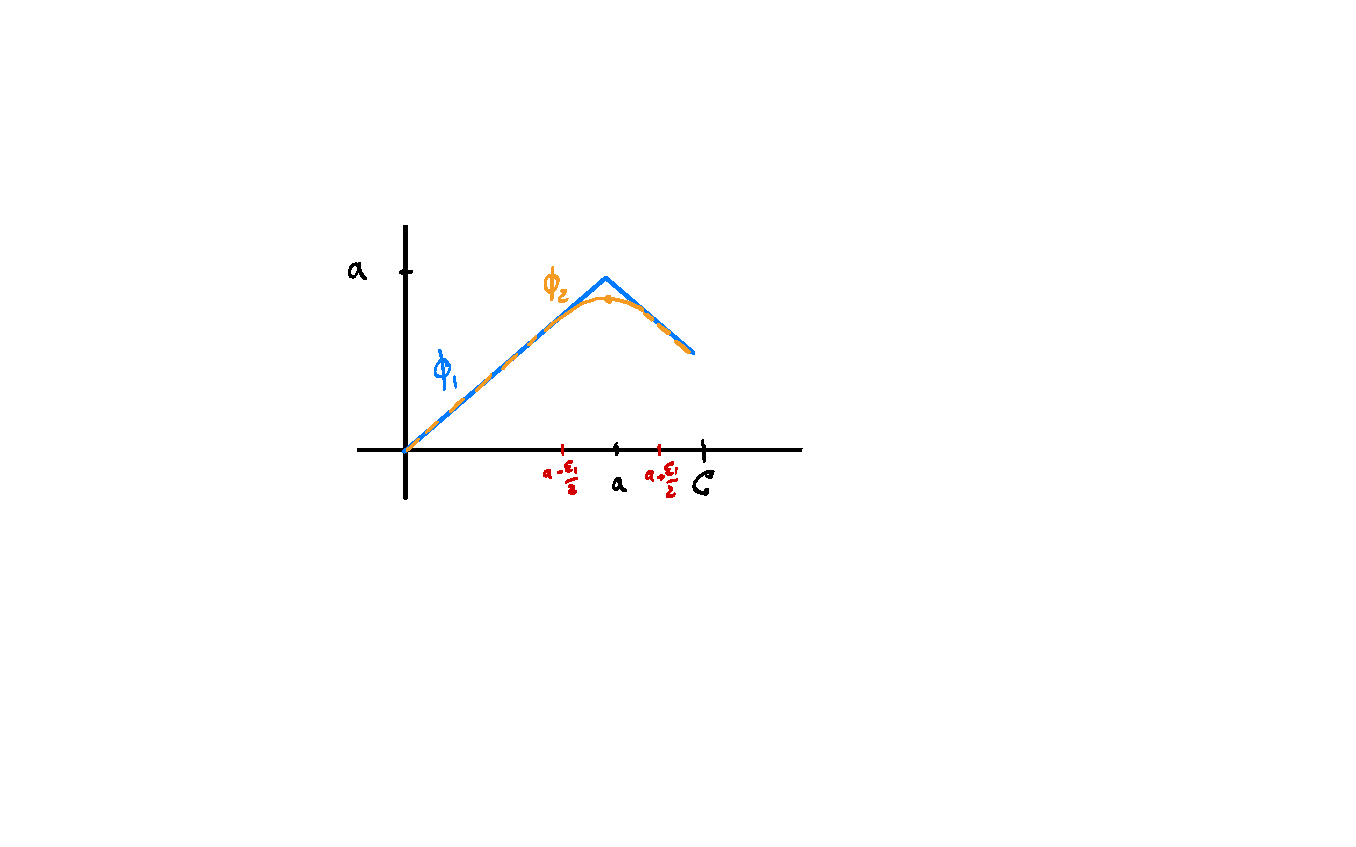
\includegraphics[scale=0.9]{first-fold.pdf}
  \centering
  \caption{The graphs of the functions $\phi_{1}$ and $\phi_{2}$.} \label{fig:first-fold}
\end{figure}


 The function $\beta$ is a smooth bump function $\beta:\R\to [0,1]$, which vanishes outside
$( a-\varepsilon_{1}, a+\varepsilon_{1})$ is increasing on $(a-\varepsilon_{1}, a)$, decreasing on $(a, a+\varepsilon_{1})$
and $\beta(a)=1$. The function $f_{W_{1}}: W_{1}\to \mathbb{R}$ is obtained through the inductive hypothesis, by applying  the Proposition to $W_{1}$. More precisely, we 
fix on $W_{1}$ the metric induced from $\mathtt{g}$ and construct the function $f_{W_{1}}$ such that it is Morse, with minimal value equal to $0$, and with maximal value $C_{1}< \xi$, and 
with $||df_{W_{1}}(z)||\geq 2\delta$, outside the union of balls $\hat{B}_{\eta_{z}}(z)$, $\eta_{z}\leq \eta$, for each critical point $z$ of $f_{W_{1}}$. The notation $\hat{B}_{-}(-)$
 indicates that the respective balls are in $W_{1}$. It is easy to see that by adjusting conveniently
 the profiles of the functions $\phi_{2}$ and $\beta$ we may ensure the desired properties for
 $f_{2}$. Notice that the critical points of $f_{2}$ are of two types,  critical points of $f_{1}$,
 and critical points of $f_{W_{1}}$,  with their Morse index raised by $1$ when viewed
 as critical points of $f_{2}$.
 
 \
 
 We will now apply this folding construction for not just one hypersurface such as $W_{1}$ before but for more hypersurfaces at the same time. First, recall the constant $K$ in the statement of the proposition and  fix a natural number  $l$ such that $ \frac{B+3\mu/2}{2^{l}}<K/4$. 

We consider a function $f_{0}$ as in the shrinking procedure and apply that construction for $\eta < \frac{B}{2^{l+1}\delta}$. We denote by $f_{1}$ the resulting function.

Consider the interval $J_{i}=[f_{1}(z_{i}), f_{1}(z_{i+1})]$, $0\leq i < m-1$, 
and divide it into $2^{l}$ equal pieces denoted
$I_{k,i}=(f_{1}(z_{i})+\frac{k S_i}{2^{l}}, f_{1}(z_{i})+\frac{(k+1)S_{i}}{2^{l}})$
where $S_{i}= f_{1}(z_{i+1})-f_{1}(z_{i})$.
Consider a continuous function:
$\varphi_{i}: J_{i}\to [0,\infty)$ with the following properties: 
\begin{itemize}
\item[-] $\varphi_{i}$ is  smooth  on each of the intervals  $I_{k,i}$ for $k=0, 1,\ldots 2^{l}-1$, with constant slope equal to $+1$ on $I_{k,i}$  when  $k$ is even and with slope equal to $-1$ when $k$ is odd. 
\item[-] We let $a_{k,i}= \frac{kS_{i}}{2^{l}}$,  $0<k\leq 2^{l}-1$. The minimal value of ${\varphi}_{i}$ is $0$ and is attained at the points $a_{k,i}$ with 
$k$ even. The maximal value of ${\varphi}_{i}$ is $\frac{S_{i}}{2^{l}}$ and is attained at the points $a_{k,i}$ with $k$ odd.
\end{itemize}
Given that $S_{i}\geq B$ we have $S_{i}/2^{l}\geq B/2^{l}>2\eta \delta$. This implies by (\ref{eq:fone'}) that all the values $a_{k,i}$ are regular values
for $f_{1}$ and that the hypersurfaces $W_{k,i}=f^{-1}(a_{k,i})$ do not 
intersect $B_{\eta}(z_{i})$ and $B_{\eta}(z_{i+1})$. We  piece together
the functions ${\varphi}_{i}$ to a new continuous function $\hat{\phi}_{1}$
defined as follows: $\hat{\phi}_{1}$ is equal to $\varphi_{i}$ on each 
interval $J_{i}$ for $i$ even and is equal to $-\varphi_{i}$ on the intervals
$J_{i}$ for $i$ odd. This means that the function $\hat{\phi}_{1}$ is smooth
at each value $f(z_{i})$, with slope alternating between $+1$ and $-1$, depending 
on the parity of $i$. Moreover, the hypersurfaces $W_{k,i}$ do not intersect
any of the balls $B_{\eta}(z)$, $z\in Crit(f_{1})$. Finally, the variation of 
$\hat{\phi}_{1}$ is at most $2 \max {\frac{S_{i}}{2^{l}}}\leq 2\frac{B+3\mu/2}{2^{l}}<K/2$, see Figure \ref{fig:saw}.
\begin{figure}
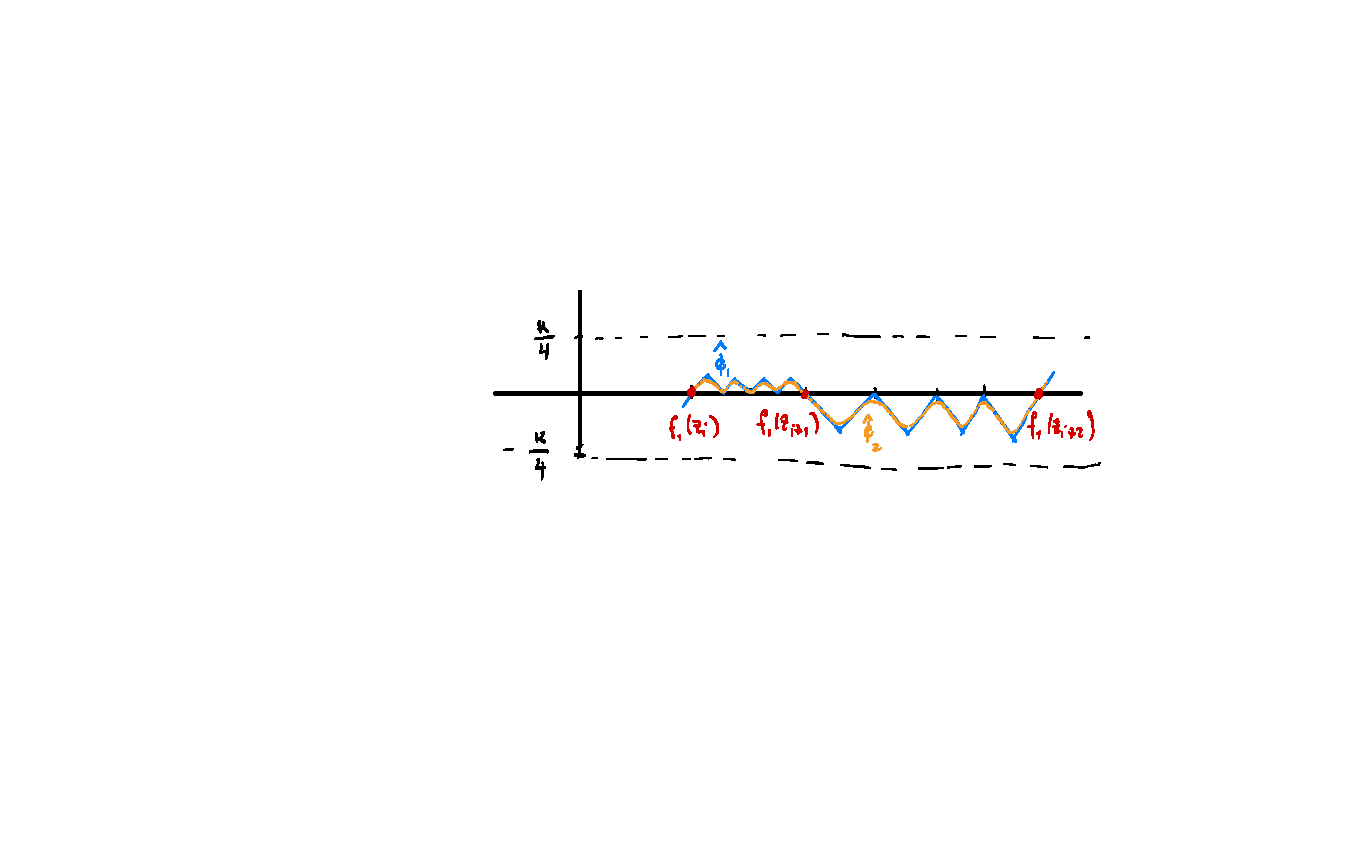
\includegraphics[scale=1.3]{saw.pdf}
  \centering
  \caption{The graphs of the functions $\hat{\phi}_{1}$ and $\hat{\phi}_{2}$.} \label{fig:saw}
\end{figure}



Next, we consider a Morse smoothing $\hat{f}_{2}$ of $\hat{\phi}_{1}\circ f_{1}$ that coincides
with $\hat{\phi}_{1}\circ f_{1}$ except on the sets 
$K_{\varepsilon_{2}, a_{k,i}}=f^{-1}_{1}([a_{k,i}-\varepsilon_{2}, a_{k,i}+\varepsilon_{2}])$. More precisely, $\hat{f}_{2}$
is given by a formula similar to (\ref{eq:perturb}) with some straightforward modifications:  the place of $\phi_{2}$ is taken
by a Morse smoothing $\hat{\phi}_{2}$ of $\hat{\phi}_{1}$ with maxima at $a_{k,i}$ for $ki$ odd, and minima
at $a_{k,i}$ for $ki$ even; on each $K_{\varepsilon_{2}, a_{k,i}}$ the place of the function $f_{W_{1}}$ is taken by a corresponding 
function $f_{W_{a_{k,i}}}: W_{a_{k,i}}\to \mathbb{R}$ of variation smaller than $\frac{S_{i}}{2^{l+1}}$; the bump function
$\beta:\R\to [-1,1]$ is supported in the union of the intervals $(a_{k,i}-\varepsilon_{2}, a_{k,i}+\varepsilon_{2})$, it is monotone on each of the intervals $(a_{k,i}-\varepsilon_{2}, a_{k,i})$ and $(a_{k,i}, a_{k,i}+\varepsilon_{2})$, it attains its maximum equal
to $1$ at the points $a_{k,i}$ for $ki$ odd and its minimum, equal to $-1$, at the points $a_{k,i}$ for $ki$ even ($0< k \leq 2^{l}-1$, $0\leq i < m-1$). 

As a result of all these choices the function $\hat{f}_{2}$ has a variation bounded from above by $K$ and the function $\varphi_{N,K,\delta}$ in the statement is defined
by adding a constant to $\hat{f}_{2}$ such that the resulting
function, denoted $\varphi_{N,K,\delta}$, is positive, with minimal value equal to $0$ and with a maximum value smaller than $K$. This function satisfies the other properties claimed in the statement.
\end{proof}

\begin{rem}\label{rem:conf_metric} In the arguments appearing later in the paper it is useful to assume, in addition to the properties in Proposition \ref{prop:Morse}, that the norm $||d\varphi_{N,K,\delta}||\leq 1$ over all of $N$. This is not so easy to achieve while keeping the metric $\texttt{g}$ fixed. However, it will be enough for us that there is a metric 
$\bar{\texttt{g}}$ on $N$, conformal to $\texttt{g}$, with $\bar{\texttt{g}}=\alpha \texttt{g}$, with $\alpha:N\to [1,\infty)$ such that the rest of the properties claimed in the proposition remain true, relative to $\bar{\texttt{g}}$,
and in addition $||d\varphi_{N,K,\delta}||_{\bar{\texttt{g}}}\leq 1$.  This is very easy to see, by adjusting the metric $\texttt{g}$, outside the neighbourhoods $B_{\eta_{z}}(z)$, at those points $x\in N$ where the norm $||d\varphi_{N,K,\delta}(x)||$ (in the metric $\texttt{g}$) is greater than $1$.
\end{rem}


\subsection{Review of Giroux's construction}\label{subsec:Giroux} We will review here the parts of \cite{Gir:Lef-cot} that will be relevant later on in the proof of Theorem \ref{thm:nearby}. The type of Lefschetz fibration considered (Definition 1 in \cite{Gir:Lef-cot}) is a Liouville manifold $(W, d\lambda)$ endowed
with a smooth map 
$$h\colon W\to \mathbb{C}$$
such that $h$ has the following properties: 
\begin{itemize}
\item[1.] The singularities of $h$ are of the form 
$$h(z)=h(0)+\sum_{j}z^{2}_{j} $$ in coordinates $(z_{1},\ldots, z_{n})$ centered at the singularity and in which $\omega=d\lambda$ is a positive $(1,1)$ form at $0$.
\item[2.] The distribution $\ker  dh \subset TW$ consists of symplectic subspaces and the singular connection provided by its symplectic orthogonal complement is complete.
\item[3.]  The manifold $W$ is exhausted by Liouville domains $(W_{k}, \lambda|_{W_{k}})$ such that for
every $w\in \mathbb{C}$ and for all sufficiently large $k\geq k_{w}$, the fiber $F_{w}=h^{-1}(w)$
intersects $\partial W_{k}$ transversely along a positive contact submanifold of $\partial W_{k}$, and
the Liouville field on $F_{w}$ dual to $\lambda|_{F_{w}}$ is complete.
\end{itemize}

The main result in Giroux's paper is the following.

\begin{thm}\label{thm:gir}[Giroux \cite{Gir:Lef-cot}] Let $N$ be a closed manifold, $\varphi:N\to \mathbb{R}$ a Morse function and $\nu$ an adapted gradient of $\varphi$ satisfying the Morse-Smale condition. Then $\varphi$ extends to a Lefschetz fibration (in the sense above) $h=f+i g\colon T^{\ast}N\to \mathbb{C}$ whose imaginary part is the function:
$$ g\colon T^{\ast}N\to \mathbb{R}\ ,\  (q,p) \mapsto\ g(q,p):=  \langle p, \nu (q)\rangle$$
and whose real part $f$ coincides with $\varphi$ on the $0$-section and is homogenous of degree $1$ in the variable $p$ near infinity.
\end{thm}

A vector field $\nu$ is called adapted to $\varphi$ if $d\varphi(\nu) >0$ away from the critical points of $\varphi$ and near each critical point $a$ there exists
a local coordinate chart that expresses $\varphi$ in Morse form, $\varphi(x)=\varphi(a)+\sum_{j} \varepsilon_{j} x^{2}_{j}$, and $\nu$ in linear 
form, $\nu(x)=2\sum_{j}\varepsilon_{j}x_{j}\partial_{x_{j}}$, $\varepsilon_{j}\in \{-1,+1\}$.

In our case, it is convenient to assume that $\nu$ is an actual gradient 
vector field of $\varphi$ with respect to a riemannian metric $\texttt{g}$ on 
$M$, \begin{equation}\label{eq:nu-grad}
\nu= grad _{\texttt{g}}(\varphi)~.~
\end{equation}
We will also assume that each critical point of $\varphi$ is unique on its critical level.

A few properties of Giroux's construction are important in our proof and we will review them now.

\begin{itemize}
\item[i.] The function $f:T^{\ast}N\to \mathbb{R}$ has the form $f=f_{0}+f_{1}$ with: 

\begin{equation}\label{eq:expression_re}
f_{0}(q,p)=\varphi(q)-\frac{1}{2}\nabla^{2}\varphi (q)(p,p)~.~
\end{equation}
Here $\nabla^{2}\varphi (q)$ is the  covariant second derivative of $\varphi$ at $q$ viewed as bilinear map on $T^{\ast}N$. The function $f_{1}:T^{\ast}N\to \mathbb{R}$ is supported away from the $0$ section $N\subset T^{\ast}N$. The precise construction of this perturbative term  $f_{1}$ requires much of the effort in \cite{Gir:Lef-cot}. Our notation is somewhat different from Giroux's and, to facilitate the correspondence
between the two papers, we indicate the differences here - our function $f_{0}$ is denoted $f^{0}$ in \cite{Gir:Lef-cot} and the function $f_{1}$ here has the form:
$$ f_{1}= \tau_{1} f^{1} - (1-\tau_{0}) f^{0}$$
where the notation on the right side of the equality is that in \cite{Gir:Lef-cot}. Namely, $\tau_{i}$ are functions only depending on the radial distance $r$ from the $0$-section such that $\tau_{1}$ vanishes for small values of $r$ and equals a large positive constant $C$ for $r$ large enough, while $\tau_{0}$ equals $1$ for small $r$  and vanishes away from the $0$-section. The function $f^{1}$ is of the form $f^{1}=r f^{\infty}$ and $f^{\infty}$ is a well chosen function defined on the sphere cotangent bundle $f^{\infty}:ST^{\ast}N\to \R$.

\item[ii.] The only critical points of $h$ are along the $0$ section and they
coincide with the critical points of $\varphi$.

\item[iii.] For each critical point $a\in Crit(\varphi)$, the vertical thimble  along the vertical straight half-line originating at $h(a)$ and pointing upwards coincides with the  unstable manifold of the Hamiltonian vector field  $X^{f}$  at $a$.

\item[iv.] The Poisson bracket $\{f, g\}$ is positive at each point $x\in T^{\ast}(N)\backslash Crit(\varphi)$ 
\end{itemize}
Our arguments require a quantitative complement to property iv which we state next:

\begin{itemize}
\item[v.] Assume that $d\varphi (\nu)\geq \delta$ outside $\cup_{a\in Crit(\varphi)}B_{\varepsilon}(a)$, for some small $\varepsilon$ such that the balls $B_{\varepsilon}(a)$, $B_{\varepsilon}(b)\subset N$ are disjoint for all $a\not=b\in Crit(\varphi)$.  
With this assumption, the construction of $f$ can be made such that 
$$\{f,g\}(x)\geq \delta,  \ \forall x\in T^{\ast}N\backslash \cup_{a\in Crit(\varphi)} B'_{\varepsilon}(a)$$
where we denote by $B'_{\varepsilon}(-)$ the respective balls of radius $\varepsilon$ in $T^{\ast}N$.
\end{itemize}

A reformulation of property v will play an important role in our argument.

\begin{cor}\label{cor:size_proj}
Under the assumptions in property \textnormal{v} above, we have that $dh(X^{f})$ is purely imaginary and $Im(dh(X^{f}(x)))\geq \delta$ for each $x\in T^{\ast}N$ outside any of the balls $B'_{\varepsilon}(a)$, $a\in Crit(h)$.
\end{cor}

Properties i, ii, iii, and iv appear explicitly in \cite{Gir:Lef-cot}. Property 
v follows easily from the proof of property iv as given in \S E \cite{Gir:Lef-cot}. To give a few more details, here are our conventions: $\omega (Y,X^{f})=df(Y)$, $\{f,g\}=\omega (X^{f},X^{g})=dg(X^{f})=-df(X^{g})$. The arguments in \cite{Gir:Lef-cot} make use of the vector field $\tilde{\nu}= -X^{g}$ that is easily seen to be a lift of $\nu$ to $T^{\ast}N$. 
It is shown that the quantity $df(\tilde{\nu})=\{f,g\}$ is positive at all points different from the critical points of $h$, which is the claim at  iv. The proof of this positivity depends on the construction of the perturbative term $f_{1}$ and appeals to a choice of the constant $C>0$ that has appeared at point i above. When this constant is taken sufficiently big, $df(\tilde{\nu})$ is  seen to be non-negative and to only vanish at the critical points of $h$. By possibly taking $C$ even bigger,  the same argument shows that property v is also true. 

Starting from property v the statement in the corollary is immediate. Indeed,
$\{f,g\}=dg (X^{f})= d(p_{2}\circ h)(X^{f})=
dp_{2}\circ (dh (X^{f}))=dh( X^{f})$ where $p_{2}:\mathbb{C}\to \R$
is the projection on the second coordinate. We have used the fact that for each
point $x$, $dh( X^{f}(x))$ is a vertical vector in $\mathbb{C}$. This is 
true because $X^{f}(x)$ is tangent to the level hypersurface  $f^{-1}(c)=(p_{1}\circ h)^{-1}(c) =h^{-1} (\{(c,y) : \ y\in \R\})$ with $c=f(x)$ and $p_{1}:\mathbb{C}\to \R$ the projection on the first coordinate. 

\subsection{Disjunction through Dehn twists}\label{subsec:Lef-Dehn} In this section we consider  Giroux's Lefschetz fibration from \cite{Gir:Lef-cot}, as recalled in \S\ref{subsec:Giroux},  and apply to it the construction in \cite{Bi-Co:lefcob-pub}, in particular the arguments in Section 4.4 in that paper.  The methods in \cite{Bi-Co:lefcob-pub}  as reflected 
in Proposition 2.3.1 (see also \S  2.3 \cite{Bi-Co:lefcob-arxiv} for more details on the relevant construction), together with the doubling of singularities in \S 4.4.2 \cite{Bi-Co:lefcob-pub} (see  Figure 17 there) applied to the Lefschetz fibration $h\colon T^{\ast}N\to \mathbb{C}$ from \S\ref{subsec:Giroux} lead to a new Lefschetz fibration $\bar{h}: E\to \mathbb{C}$ which is schematically represented in Figure \ref{fig:new_fibr}.  
\begin{figure} [h]
  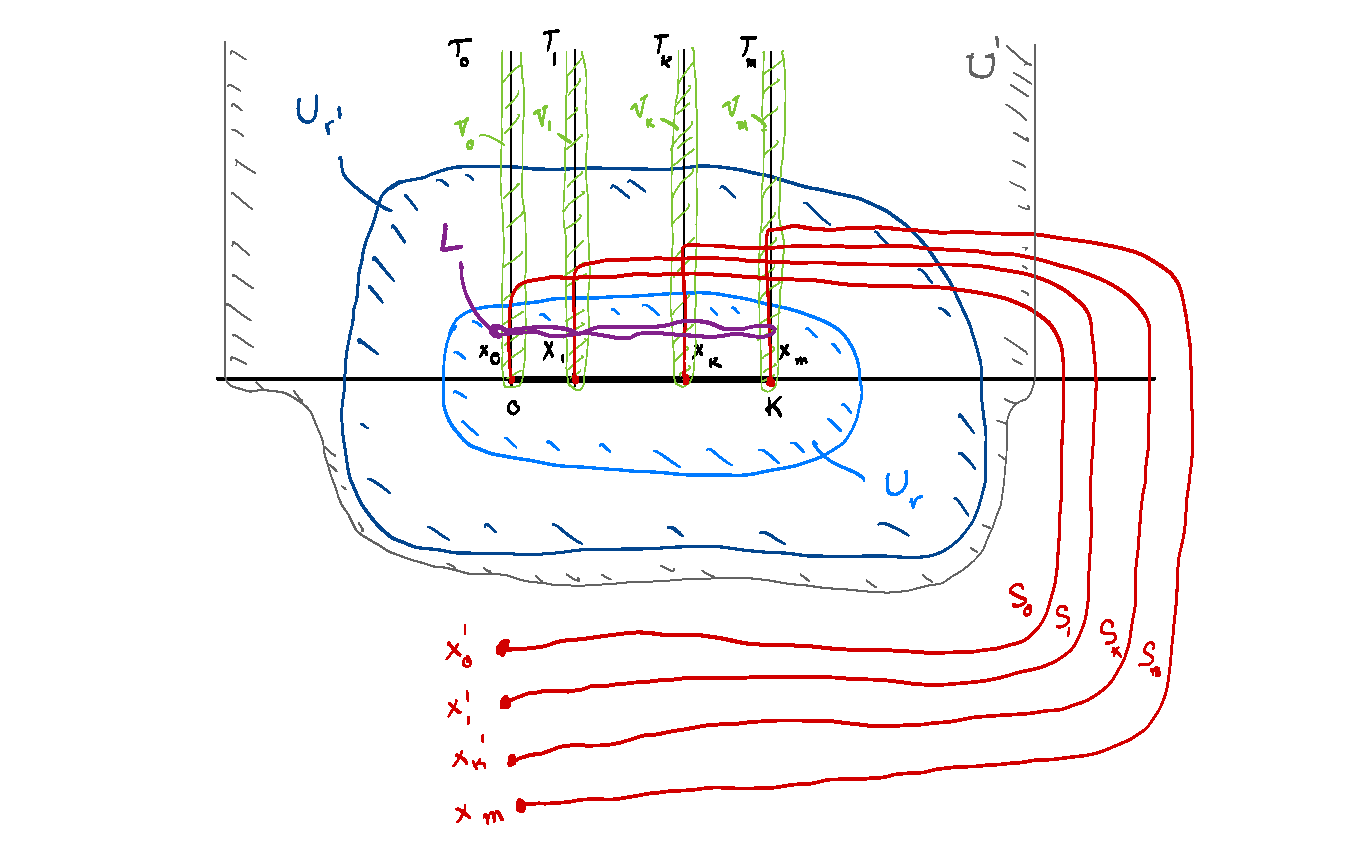
\includegraphics[scale=0.9]{new_fibr.pdf}
  \centering
  \caption{The fibration $\bar{h}:E\to \mathbb{C}$.} \label{fig:new_fibr}
\end{figure}
Here are the main relevant properties of $\bar{h}$.  We assume the setting 
in Theorem \ref{thm:gir}. In particular, we have the 
Morse function $\varphi: N\to \mathbb{R}$ with a unique critical point on each critical level and that is such that the pair $(\varphi, \texttt{g})$ is  Morse-Smale where $\texttt{g}$ is a fixed Riemannian metric on $N$ and the properties  i.-v. from \S\ref{subsec:Giroux} are satisfied. Furthermore, we have:
\begin{itemize}
\item[a.] The Morse function $\varphi: N\to \mathbb{R}$ has values in $[0,K]$, having $0$ as minimal value and $K$ for maximal value. 
\item[b.]  We put $U_{r}=h(D_{r}^{\ast}N)$  where the disk cotangent bundle  $D_{r}^{\ast}N$ is defined relative to the metric $\texttt{g}$, and 
similarly $U_{r'}=h(D_{r'}^{\ast}N)$ - both these sets are represented in Figure \ref{fig:new_fibr}.
\item[c.]  Fix a constant $R>0$ big enough such that $U_{r'}\subset [-R,R]\times\mathbb{R}$. There is a neighbourhood $U'\subset \mathbb{C}$ of $U_{r'}\cup ([-R, R]\times [0,\infty))$ such that $h$  and  $\bar{h}$ agree on $h^{-1}(U')$.
\item[d.] The fibration $\bar{h}$ has one additional critical point $x'_{i}$ for 
each critical point $x_{i}$ of $h$. For each pair $x_{i}, x'_{i}$ of such critical points, $x_{i}$ and $x'_{i}$ are related through a matching cycle $S_{i}\subset E$ (which is a Lagrangian sphere) whose image onto $\mathbb{C}$ is like in Figure \ref{fig:new_fibr}. 
\item[e.] The vertical thimbles pointing up and originating at the critical points 
$x_{i}$ are denoted by $\tau_{i}$. They are unstable manifolds of the Hamiltonian vector field $X^{\bar{f}}$ at each critical point $x_{i}$ with $\bar{f}= Re (\bar{h})$ (recall from iii. that $\bar{f}= f$ over $U'$).
\item[f.] Fix some $\delta >0$ and assume that $h= f+i g$ satisfies $\{f,g\}(x)\geq \delta$ at all points $x$ outside
small balls $B'_{\varepsilon}(x_{i})$, $x_{i}\in Crit(\varphi)$, as at point v. in \S\ref{subsec:Giroux}. Under this assumption we fix small neighbourhoods $V_{i}\subset E$  for each of the thimbles $\tau_{i}$ such that $V_{i}\supset B'_{\varepsilon}(x_{i})$. The projection of the $V_{i}$'s onto $\mathbb{C}$ is as in the picture. 
\end{itemize}
In our arguments the constants $\delta>0$, $K>0$ are fixed in advance with 
$\delta < 1$ and the function $\varphi=\varphi_{N,K,\delta}$ is given  by Proposition \ref{prop:Morse}. The key property that will be used further below in the proof is provided by Corollary \ref{cor:size_proj}: 
\begin{equation}\label{eq:Ham_big}
 \ \  d\bar{h}(X^{\bar{f}}(x))\in i [\delta,+\infty) \subset  i\mathbb{R}\subset \mathbb{C}\ \   , \forall\ x\in \bar{h}^{-1}(U')\backslash (\cup_{i} V_{i}) ~.~
 \end{equation} 
 
 We will also assume that, after possibly a conformal change of metric, as in  Remark \ref{rem:conf_metric}, passing from the arbitrary metric $\mathtt{g}$, to a conformally equivalent metric $\bar{\mathtt{g}}=\alpha \mathtt{g}$ with $\alpha:N\to [1,\infty)$, we have $||d\varphi||\leq 1$.  We will use this metric $\bar{\mathtt{g}}$ throughout from this point on and discuss this modification further below in \S\ref{subsec:general}. 
 This means that
$||\nu ||\leq 1$ - see (\ref{eq:nu-grad}) - and further implies by the description of $g$ in Theorem \ref{thm:gir} that:
\begin{equation}\label{eq:width}
U_{r}\subset \mathbb{R}\times [-r,r], \ \  \forall r \in \mathbb{R}
\end{equation} 

The description of $f_{0}$ from the point i, in \S\ref{subsec:Giroux} implies that, for $r$ sufficiently small, we  have 
\begin{equation}\label{eq:length}
U_{r}\subset [- C_{\varphi} r , K + C_{\varphi} r]\times [-r,r]
\end{equation}
where $C_{\varphi}$ is a positive constant depending on the $C^{2}$ norm
of $\varphi$.

In this context, the main result that we need from \cite{Bi-Co:lefcob-pub} is next.

\begin{prop}[\cite{Bi-Co:lefcob-pub}] \label{prop:disj}For any Lagrangian $L\subset D^{\ast}_{r}N$, and any arbitrarily small neighbourhoods $N_{i}$ of the  matching cycles $S_{i}$,  there exist models of the Dehn twists $\tau_{S_{i}}$ that are  supported in $N_{i}$ and  such that  $\tau_{S_{m}} \circ \ldots  \circ \tau_{S_{2}}\circ \tau_{S_{1}}\circ \tau_{S_{0}}(L)$ does not intersect any of the thimbles $\tau_{i}$.
\end{prop}

\subsection{Proof of Theorem \ref{thm:nearby}}\label{subsec:finish-proof}

The proof of the theorem will be completed in four steps. In \S\ref{sububsec:disjunction-we} we start from the setting in \S\ref{subsec:Lef-Dehn} and use (\ref{eq:Ham_big}), (\ref{eq:length}) and Proposition \ref{prop:disj} to show that, if $r$ is sufficiently small,  the iterated Dehn twist $$\tau_{m,\ldots, 1,0}L= \tau_{S_{m}} \circ \ldots  \circ \tau_{S_{2}}\circ \tau_{S_{1}}\circ \tau_{S_{0}}(L)$$ can be disjoined from $D^{\ast}_{r}(N)$ through a Hamiltonian isotopy of energy 
at most $8Kr/\delta$.  In \S\ref{subsec:exact-seq} we reformulate the disjunction result in Lemma \ref{lem:disj-energy} in terms of Lagrangian spheres that restrict to fibers $F_{x_{i}}\subset D^{\ast}_{r}(N)$. In \S\ref{subsubsec:back_to_alg} we establish an approximability type result in Proposition \ref{prop:estimates-in-r} that still involves the constants $K$, $r$, $\delta$. Finally, the proof concludes in \S\ref{subsec:general} where we get rid of the restriction of $r$ being sufficiently small, showing that the conformal change of metric   $\texttt{g}$ does not affect the argument and that
the constants $K$, $\delta$ in Proposition \ref{prop:estimates-in-r} can be picked as needed to deduce the statement of  Theorem \ref{thm:nearby}.
\subsubsection{Disjunction with controlled energy.}\label{sububsec:disjunction-we}
The aim in this subsection is to prove the following Lemma. To state it we fix
the constants $0<\delta < 1$, $K>0$
 and the function $\varphi=\varphi_{N,K,\delta}$ given  by Proposition \ref{prop:Morse}, just as discussed in \S\ref{subsec:Lef-Dehn}.  We
also assume that points a. - f. there are satisfied as well as the inclusions in (\ref{eq:Ham_big}) and (\ref{eq:length}). 

\begin{lem}\label{lem:disj-energy} For $r$ sufficiently small, for any (marked) exact Lagrangian $L\subset D^{\ast}_{r} N$ the iterated Dehn twist $\tau_{m, \ldots, 1,0}L$ can be disjoined from $D^{\ast}_{2r} (N)$ inside $E$ with less  than $8Kr/\delta$ energy. 
\end{lem}
\begin{proof} To simplify notation denote $L'= \tau_{m, \ldots, 1,0}L$. Recall
that the constant $C_{\varphi}$ from (\ref{eq:length}) only depends on $\varphi$. We start by choosing $r>0$ such that $rC_{\phi}<K/4$. We also pick the constant $r'$ such that $r'=2r$. Therefore,
we deduce from (\ref{eq:length}) that 
$$U_{r}\subset [-K/4, 5K/4]\times [-r,r]$$
and, similarly $$U_{2r}\subset [-K/2, 3K/2]\times [-2r,2r]~.~$$
Assume for a moment that 
\begin{equation}\label{eq:assumption-dis}
L' \subset [\bar{h}^{-1}(U') \backslash \ (\cup_{i} V_{i}) ] \cup (\cup_{i} N'_{i})
\end{equation}
where $N'_{i}\supset N_{i}$ are neighbourhoods of the matching cycles $S_{i}$, possibly slightly larger than $N_{i}$. In that case, inspecting Figure \ref{fig:new_fibr} and  using (\ref{eq:Ham_big}), we see that the Hamiltonian flow $- X^{\bar{f}}$ moves $L'$ outside of $W_{K,r}=\bar{h}^{-1}([-K/2, 3K/2]\times [-2r,\infty))$ in time 
less than $4r/\delta$. At the same time the variation of $\bar{f}$ over $W_{K,r}$ is at most $2K$. It follows  that the Hofer displacement energy
of $L'$ from $W_{K,r}$, and, in particular, from $D^{\ast}_{2r}(N)\subset W_{K,r}$ 
 is less than $8Kr/\delta$.

We now intend to show that assumption (\ref{eq:assumption-dis}) is satisfied by some Lagrangian $L''=\psi (L')$ for some Hamiltonian diffeomorphism $\psi$ that will be described next. To this purpose, we notice that the closures of the neighbourhoods $V_{i}$ of the thimbles $\tau_{i}$ are included in the interior of $W_{K,r}$. Around each thimble $\tau_{i}$ we can find a Hamiltonian isotopy $\psi_{i}$ supported in a slightly larger neighbourhood $V'_{i}\subset W_{K,r}$ that is ``repelling'' away from
the thimble $\tau_{i}$ and such that $\psi_{i}$ leaves the thimble $\tau_{i}$ invariant (as a set) and moves the intersection $L'\cap V_{i}$  outside of $V_{i}$ , without creating any new intersections with $V_{i}$. For different $i$'s these Hamiltonian isotopies have disjoint support and thus they can be incorporated in a single isotopy whose time-one map, $\psi$, has
the property that $L''=\psi (L')$ satisfies (\ref{eq:assumption-dis}). 

We next apply to $L''$ the estimate for the displacement Hofer energy relative to $W_{K,r}$. Thus, there exists a Hamiltonian isotopy $\phi$ of energy less than
$8Kr/\delta$ such that  $\phi (L'')\cap W_{K,r}=\emptyset$. As the support of
$\psi$ is inside $W_{K,r}$ we deduce that $\psi^{-1}\phi\psi (L') \cap W_{K,r}=\emptyset$ and, by the bi-invariance of the Hofer norm, we also have $||\psi^{-1}\phi\psi||_{H}=||\phi||_{H}< 8Kr/\delta$ which concludes the proof of the lemma.

\end{proof}

\begin{rem}\label{rem:small_Dehn}
Notice that, as in Proposition \ref{prop:disj}, the support of the Dehn twists can be assumed to be contained in neighbourhoods of the $\hat{S}_{i}$ that are as small as desired.

\end{rem}
\subsubsection{Replacing matching cycles by Lagrangian spheres that restrict to fibers}\label{subsec:exact-seq} In this subsection we rewrite the disjunction energy estimate from Lemma \ref{lem:disj-energy} in terms of Dehn twists where the matching cycles $S_{i}$ are replaced by perturbations  $\hat{S}_{i}$ such that the intersection of $\hat{S}_{i}$ with $D^{\ast}_{r}(N)$ coincides with the cotangent fiber $F_{x_{i}}$.

We assume that $r$ is sufficiently small such that for each 
fiber $\overline{F}_{x_{i}}\subset D^{\ast}_{r}(N)$ (we recall $\{x_{i}\}_{i}=Crit(\varphi)$)  the image $\bar{h}(\overline{F}_{x_{i}})$ is included in $V_{i}$, see 
(\ref{eq:expression_re}),  and recall the expression of $g= Im(h)$ from Theorem \ref{thm:gir}. In particular, all these images are disjoint. We then 
consider a Hamiltonian diffeomorphism $\eta$ that is supported in $D^{\ast}_{\frac{3}{2}r}(N)$ and that deforms $S_{i}\cap D^{\ast}_{r}(N)$ to $F_{x_{i}}$. We will 
assume that the ``bends'' of $S_{i}$ in Figure \ref{fig:new_fibr} take place 
outside of $D^{\ast}_{\frac{3}{2}r}(N)$. We denote $\hat{S}_{i}=\eta(S_{i})$. We may also assume that $\eta$ is constructed such that $\hat{S}_{i}\cap D^{\ast}_{r}(N) = \overline{F}_{x_{i}}$ and $\eta(D^{\ast}_{r}(N))= D^{\ast}_{r}(N)$. Constructing such an $\eta$ is a simple exercise  by comparing the local expressions of the fiber $x_{i}$ and that of the thimble
$\tau_{i}$. Obviously, the submanifolds $\hat{S}_{i}$ are also Lagrangian spheres and we pick models for the Dehn twists relative to $\hat{S}_{i}$ such 
that $\tau_{\hat{S}_{i}}=\eta \circ \tau_{S_{i}}\circ \eta^{-1}$. This means, in particular,
that for any Lagrangian $L\subset D^{\ast}_{r}(N)$ we can write: 
$$\tau_{\hat{S}_{i}}(L)= \eta ( \tau_{S_{i}} (\eta^{-1}(L)))~.~$$
By iterating this relation we deduce that the iterated Dehn twist
$$\hat{\tau}_{m,\ldots, 1,0} (L) = \tau_{\hat{S}_{m}}\circ \ldots  \circ \tau_{\hat{S}_{1}}\circ\tau_{\hat{S}_{0}} (L)$$
satisfies
$$\hat{\tau}_{m,\ldots, 1,0} (L) =\eta( \tau_{m,\ldots,1,0} (\eta^{-1}(L))~.~$$
We know from the proof of Lemma \ref{lem:disj-energy} that there exists a Hamiltonian diffeomorphism $\phi'$ that, for any Lagrangian $L''$ (in our class), displaces $\tau_{m,\ldots,1,0}(L'')$ from $W_{K,r}$ and is of energy less than $8Kr/\delta$.  For a fixed Lagrangian $L$ we apply this property to $L''=\eta^{-1}(L)$  and, using the fact that the support of $\eta$ is included in $W_{K,r}$, we deduce that $\eta \circ \phi'\circ \eta^{-1}$ displaces $\hat{\tau}_{m,\ldots, 1, 0}(L)$ from  $W_{K,r}$. The Hofer norm of $\eta\circ \phi'\circ \eta^{-1}$ equals that of $\phi'$ and is thus smaller than $8Kr/\delta$.
In summary:
\begin{prop}\label{lem:disj_fibers} With the notation above, and for $r$ sufficiently small,  the conclusion  of Lemma \ref{lem:disj-energy} also applies to the iterated Dehn twist $\hat{\tau}_{m,\ldots, 1,0}(L)$ with each Dehn twist $\tau_{\hat{S}_{i}}$ having support in a neighbourhood of $\hat{S}_{i}$ that can be assumed as small as desired. \end{prop} 


\subsubsection{Translating geometry into algebra}\label{subsubsec:back_to_alg}
In this section, we interpret the geometric disjunction result in 
Proposition \ref{lem:disj_fibers} in homological terms in
a Fukaya TPC  system $\widehat{\msc}(D^{\ast}_{r}(N))$.
The purpose here is to translate homologically the statement in Proposition \ref{lem:disj_fibers}. 
Two systems of related Fukaya categories will be important for us here, with components associated with the perturbation choice $p\in\mathcal{P}$ as below:
\begin{equation}\label{eq:components_cat}
\fuk(\mathcal{L}ag^{(ex)}(D^{\ast}_{r}N), p)\hookrightarrow \fuk(\mathcal{L}ag^{(ex)}E,p)~.~
\end{equation}
The category on the left is the one appearing in \S\ref{subsec:back} and the one on the right is
constructed just as in Chapter \ref{ch:ffuk}. Its objects are marked exact, closed Lagrangian submanifolds in
$E$, the total space $E$ of the Lefschetz fibration  from \S\ref{subsec:Lef-Dehn}. An important point has to do with the choice of perturbations $p$: they are first picked on $D^{\ast}_{r}N$ and then extended to $E$. This is why there is an inclusion of $A_{\infty}$-categories relating the two sides. These categories fit into systems of filtered $A_{\infty}$-categories as in \S\ref{sb:sys-ainfty}. Further, as in \S\ref{sb:sys-fuk}, we 
obtain the system of TPCs $\widehat{PD}(\fuk(\mathcal{L}ag^{(ex)}(E))$. We also have the system of TPCs from \S\ref{subsec:back}, $\widehat{\msc}(D^{\ast}_{r}N) =(\msc_{p}(r), \mathcal{H}_{p,q})$. Notice that we include in the notation the radius $r$ of the relevant disk bundle. The categories $\msc_{p}(r)$ are homotopy categories of filtered  modules over the filtered Fukaya category $\mathcal{A}_{p}(r)=\fuk(\lagex(D^{\ast}_{r}N); p)$ and we have an inclusion of 
TPCs: $$ J_{p,r}:\msc_{p}(r)\hookrightarrow  H(F\md_{\mathcal{A}_{p}(r)})~.~$$

Because the perturbations on $E$ extend the perturbations on $D^{\ast}_{r}N$, the inclusion (\ref{eq:components_cat}) induces  
 pull-back TPC functors:
%$$\xi:\widehat{PD}(\fuk(\mathcal{L}ag^{(ex)}(E)) \to \widehat{\msc}(D^{\ast}_{r}N) $$
$$\xi_{p}:PD(\fuk(\mathcal{L}ag^{(ex)}(E), p)) \to H(F\md_{\mathcal{A}_{p}(r)})~.~$$
These functors commute with the comparison functors $\mathcal{H}_{p,q}$ if we  choose the perturbations used to define the comparison $\mathcal{H}_{p,q}$ functors for $D^{\ast}_{r}N$ by restriction of the perturbations used to define the corresponding functors for $E$. Notice also that, because the Lagrangian spheres $\hat{S}_{i}$ from \S\ref{subsec:exact-seq} intersect 
$D^{\ast}_{r}N$ along the fibers $\overline{F}_{x_{i}}$ it follows
that the module $F_{x_{i}}$ corresponding to the fiber $\overline{F}_{x_{i}}$ (see \S\ref{subsec:back}) is the pull-back of the Yoneda module $\mathcal{Y}(\hat{S}_{i})$. In particular, this module belongs to the image of $J_{p,r}$.  In $E$, the comparison functors $\mathcal{H}_{p,q}$ preserve the (Yoneda) modules associated with $\hat{S}_{i}$ for $p\preceq q$ and thus we deduce that, with these choices of perturbations, the family
$\mathcal{F}=\{F_{x_{i}}\}_{i}$ satisfies property ($\ast$)
from  the statement of Theorem \ref{thm:nearby}.
The next result brings us very close to the statement of this  theorem .

\begin{prop}\label{prop:estimates-in-r}
Assuming the setting and notation above, for $r$ sufficiently small and for a choice of perturbations $p$ with $\nu(p)$ sufficiently small, any exact, marked Lagrangian $L\subset D^{\ast}_{r}(N)$ satisfies in $\msc_{p}(r)$:
$$d_{int}\left( L, \Ob\  \langle\{F_{x_{0}},\ldots, F_{x_{m}}\} \rangle^{\Delta}\right) \leq 48 Kr/\delta~.~$$  
\end{prop}

\begin{proof} To simplify notation denote in this proof $c= 8Kr/\delta$, and 

\begin{equation} \label{eq:amb_Fuk}
\mathscr{D}_{p}(E):=PD(\fuk(\mathcal{L}ag^{(ex)}(E), p))~.~
\end{equation}

We first notice that to prove the claim it is enough to show:
\begin{lem}\label{lem:in_large} There are strict exact, weighted triangles in
$\mathscr{D}_{p}(E)$ of the form:
\begin{equation}\label{eq:iterated_cones1}
\Delta_{i} \ : \ Z_{i}\longrightarrow X_{i}\longrightarrow X_{i+1} \  , \ 0\leq i \leq m-1
\end{equation}
 such that $X_{0}$ is the Yoneda module of a Lagrangian disjoint from $D^{\ast}_{r}N$,  $ X_{m}= L$, and with the $Z_{i}$ of the form $\Sigma^{p(i)}\hat{S}_{x_{q(i)}}$ for some integers $p(i), q(i)$,  or possibly $Z_{i}=0$, and of total weight not more than $3c$. 
\end{lem}


Indeed, in that case, by the construction in Lemma 2.87
in \cite{BCZ:tpc} we obtain that there is a similar sequence  of triangles
\begin{equation*}\label{eq:iterated_cones2}
\Delta'_{i} \ : \ Z'_{i}\longrightarrow X'_{i}\longrightarrow X'_{i+1}
\end{equation*}
with $Z'_{j}$ again of the form $\Sigma^{l(j)}\hat{S}_{x_{s(j)}}$ or $=0$,
 with each $\Delta'_{i}$  exact in
 $(\mathscr{D}_{p}(E))^{0}$, with, $X'_{0}=X_{0}$, and with the last term $X'_{m}$ carrying a $6c$-isomorphism $X'_{m}\to L$. This means
by Lemma 2.85  \cite{BCZ:tpc} that $d_{int}^{\mathscr{D}_{p}(E)}(L,X'_{m})\leq 6c$. We now pull-back the triangles 
$\Delta'_{i}$ to  $H(F\md_{\mathcal{A}_{p}(r)})$. This produces triangles: 
$$
\Delta''_{i} \ : \ Z''_{i}\longrightarrow X''_{i}\longrightarrow X''_{i+1}
$$
that are exact in $(H(F\md_{\mathcal{A}_{p}(r)}))^{0}$, with $X''_{0}=\xi_{p}(X'_{0})=0$, with $Z''_{j}$ of the form
$\Sigma^{l(j)}F_{x_{s(j)}}$ (or $=0$) and with $\dint (X''_{m},L)\leq 6c$. Given that $\msc_{p}(r)$ contains the triangular completion of all the fiber modules $F_{x_{i}}$ we deduce that $X''_{i}\in \Ob (\msc_{p}(r))$ for all $i$ and this ends the proof of 
the Proposition \ref{prop:estimates-in-r} up to showing the Lemma \ref{lem:in_large}.
\end{proof}

\begin{rem} \label{rem:pull}
It is useful to emphasize that the pull-back $\xi_{p}$ is not necessarily full and faithful. In particular, 
 $\xi_{p}: HF(\hat{S}_{x_{i}},\hat{S}_{x_{j}})\to \hom_{\msc_{p}(r)}(F_{x_{i}}, F_{x_{j}})$ is not necessarily either injective nor surjective.
\end{rem}

\begin{proof}[Proof of Lemma \ref{lem:in_large}]
To construct the desired sequence of strict exact triangles we first fix the notation
$L_{m+1}=L$,  $L_{m-i}=\tau_{\hat{S}_{i}}(L_{m-i+1})$ so that $L_{0}=\hat{\tau}_{m,\ldots, 1,0}(L)$.
The statement of Proposition \ref{lem:disj_fibers} shows that $L_{0}$ can be  disjoined from $D^{\ast}_{r}(N)$ by a Hamiltonian isotopy $\Phi$ of Hofer norm $||\Phi||_{H} < c=\frac{8Kr}{\delta}$. 
By taking $p$ such that $\nu(p) \ll c- ||\Phi||_{H}$ we deduce, in TPC terminology,  that there is a weighted strict exact triangle in $\mathscr{D}_{p}(E)$:
\begin{equation}\label{eq:first-ex} 
0\longrightarrow L_{0}' \longrightarrow L_{0}\longrightarrow 0
\end{equation}
of weight $2c$, with $L_{0}'$ the Yoneda module of a Lagrangian  $L'_{0}\subset E$ disjoint from $D^{\ast}_{r}(N)$. This will be taken as the first triangle in our sequence (in other words we take $X_{0}=L_{0}'$). 

To construct the next triangles, 
we consider the homological interpretation of the Dehn twist, as
in Seidel's work  \cite{Se:book-fukaya-categ}, with the exception that we want to express the output  in a persistence context.  
Namely, we claim that in $\mathscr{D}_{p}(E)$ we have weighted strict exact triangles
\begin{equation}\label{eq:exact-tr}\hat{S}_{x_{m-i}}\otimes HF(\hat{S}_{x_{m-i}}, L_{i})\longrightarrow L_{i-1}\longrightarrow L_{i}~.~
\end{equation}
Here the Floer homology group $HF(\hat{S}_{x_{m-i}},L_{i})$ is a persistence module and the tensor product is a tensor product in the persistence realm. Moreover, to avoid complicating the notation, we identify the Lagrangians $L_{i}$ with their associated filtered Yoneda modules. 

The  triangle (\ref{eq:exact-tr}) is a persistence refinement of  Seidel's
classical Dehn-twist exact triangle.  This refinement is a strict exact triangle in the terminology of TPC's, of a weight denoted by $\varepsilon_{i}$ (see \cite{BCZ:tpc}) and, additionally, $\varepsilon_{i}$ depends on the size of the support of the Dehn twist $\tau_{\hat{S}_{i}}$, and can thus be made arbitrarily small.  This  feature of (\ref{eq:exact-tr})  can be seen most easily through the cobordism approach to the Dehn twist  due to Mak-Wu \cite{Mak-Wu:Dehn-twist} which, combined with the Lagrangian cobordism results in \cite{Bi-Co-Sh:LagrSh}, provides an upper bound for the weight of the triangle in terms of the shadow of the cobordism constructed in \cite{Mak-Wu:Dehn-twist}. This shadow can be made as close to $0$ as needed by diminishing the  neighbourhood of $\hat{S}_{i}$ that contains the support of $\tau_{\hat{S}_{i}}$.

To proceed, we pick the Dehn twists $\tau_{\hat{S}_{i}}$ with
sufficiently small support such that the weights $\varepsilon_{i}$ of the triangles
(\ref{eq:exact-tr}) sum up to less than $c$.  We now notice that the persistence module $HF(\hat{S}_{x_{m-i}}, L_{i})$ can be viewed as the homology of a direct sum  $S$ of (translates of) elementary filtered complexes
$E_{2}(a, b)=\k(a, b:  da=0, db=a)$ and $E_{1}(c)=\k(c : dc=0)$ with the generators $x$ in both cases filtered with values $v(x)\in \R$, and $v(b)> v(a)$. The generators have degrees $0$ for $a$ and $c$, and $1$ for $b$.
The first type of filtered module can be written as a cone
$$E_{2}(a,b)=Cone \left( E_{1}(b)[-1]\to  E_{1}(a) \right)$$ over the obvious isomorphism, $b\to a$. Making use of this decomposition of $HF(\hat{S}_{x_{m-i}}, L_{i})$, the triangle (\ref{eq:exact-tr})
can be refined to a sequence of exact triangles in $(\mathscr{D}_{p}(E))^{0}$ of the form
\begin{equation}\label{eq:tr-ref}
\Delta_{i,j} \ \ \ : \ \ \ \hat{S}_{x_{i}}\otimes  E_{1}(d_{j})\to L_{i,j}\to L_{i,j+1}
\end{equation}
for $0\leq j\leq m(i)$
where $L_{i,0}=L_{i}$ and $d_{j}$ is one of the generators of type $a,b, c$ that appear in the sum $S$, followed by a last strict exact triangle of weight $\varepsilon_{i}$ of
 the form 
 $$0\longrightarrow L_{i,m(i)}\longrightarrow L_{i+1}~.~$$
 This refinement is an immediate consequence of the octahedral axiom.

Notice that $\hat{S}_{x_{i}}\otimes E_{1}(x)$ is isomorphic to
$\Sigma^{v(x)}\hat{S}_{x_{i}}$. Therefore, by splicing together
all these exact triangles, starting with (\ref{eq:first-ex}) and following in order with $\Delta_{0, j}$, $0\leq  j\leq m(0)$ followed by   $\Delta_{1,j}$, \ $0\leq  j \leq m(1)$ and so forth, we obtain a sequence of exact triangles of the form required and of total weight not more than $3c$ which concludes the proof of the Lemma.
\end{proof}


\subsubsection{Conclusion of the proof.}\label{subsec:general} 
Theorem \ref{thm:nearby} is formulated in terms of the unit disk
bundle $D^{\ast}N$ with respect to some metric $\mathtt{g}$ but 
Proposition \ref{prop:estimates-in-r} is established for a disk bundle
$D^{\ast}_{r}N$ with $r$ small and with respect to a metric 
$\overline{\mathtt{g}}$ that is conformally equivalent to $\mathtt{g}$, as at the end of \S\ref{subsec:Lef-Dehn}.
 
To show Theorem \ref{thm:nearby} it suffices to show that for {\em any $r$}, and {\em any} metric $\mathtt{g}$ and any $L\subset D^{\ast}_{r}(N)$ we have 
 $$d_{int}(L, \Ob \langle \mathcal{F}_{\varepsilon}
 \rangle^{\Delta})) < \varepsilon+c_{\varepsilon}\nu(p)$$ where $\mathcal{F}_{\varepsilon}$ is a finite family of (modules of) fibers  depending on $\varepsilon$ and on $r$. The interleaving distance $d_{int}(-)$ is defined on the 
 triangulated persistence category $\msc_{p}(r)$ for the perturbation parameter $p$ such that $\nu(p)$ is small enough. Moreover, these perturbation parameters, and the respective TPCs, are supposed to fit into a coherent family of TPCs as in Definition \ref{d:approx-sys} and 
 the assumption ($\ast$) from Theorem \ref{thm:nearby} should be satisfied.
  
  \
  
 We fix $\varepsilon > 0$ and the metric $\mathtt{g}$. We keep the constant $0<\delta < 1$ as in the previous subsections.  
 We intend to use  Proposition \ref{prop:estimates-in-r}. We need to address the following points: 
 \begin{itemize}
 \item[i.] The proposition applies to the metric $\bar{\mathtt{g}}=\alpha \mathtt{g}$ with $\alpha:N\to [1,\infty)$ (chosen such  that we have $||d\varphi||\leq 1$, see Remark \ref{rem:conf_metric}) and not directly to $\mathtt{g}$.
 \item[ii.] The proposition applies to only values of $r$ that are sufficiently small.
 \end{itemize}
 
 For i. we denote by $|| - ||_{\mathtt{g}}$ and respectively by
 $||-||_{\bar{\mathtt{g}}}$ the norms with respect to the two metrics and 
 notice that for $a\in T^{\ast}(N)$ we have $||a||_{\bar{\mathtt{g}}}=\frac{1}{\sqrt{\alpha}}||a||_{\mathtt{g}}$. As a result $D^{\ast}_{r,\mathtt{g}}(N)\subset D^{\ast}_{r, \bar{\mathtt{g}}}(N)$ (where we add the metrics in the notation for the respective disk bundles).  Therefore,  the statement for the metric $\bar{\mathtt{g}}$ implies automatically  the corresponding result for the metric $\mathtt{g}$. 
 
 \
 
 It remains to discuss  point ii.  We want to show the statement for an arbitrary  value $R>0$. We pick $K>0$ such that  $48 K R/\delta \leq \varepsilon$ and a Morse function $\varphi=\varphi_{N,K,\delta}$, as in Proposition \ref{prop:Morse}.  This determines the family $\mathcal{F}_{\varepsilon}$ of fibers $F_{x_{i}}$, one for each critical point $x_{i}$ of $\varphi$.  We also consider the metric $\bar{\mathtt{g}}=\alpha \mathtt{g}$ obtained from $\mathtt{g}$ by rescaling as in Remark \ref{rem:conf_metric} with $\alpha :N\to [0,\infty)$ such that with respect to $\bar{\mathtt{g}}$ we have $||d\varphi||\leq 1$.

In case $R$ is small enough, the statement of Proposition  \ref{prop:estimates-in-r} directly applies and there is nothing further to prove. Assuming this is not the case, consider a sufficiently small $r$ such that the estimate in the statement of Proposition  \ref{prop:estimates-in-r}
\begin{equation}\label{eq:ineq3}d_{int}(L, \ \Ob \langle \{F_{x_{0}},\ldots, F_{x_{m}}\} \rangle^{\Delta} ) \leq 48 Kr/\delta 
\leq \varepsilon \frac{r}{R}\end{equation}
is valid in $\msc_{p} (r)$ - the TPC associated with the exact, marked Lagrangians in $D^{\ast}_{r, \bar{\mathtt{g}}}(N)$ with respect
to perturbation data $p$ with $\nu(p)$ sufficiently small.
 
We consider the following rescaling map $\psi_{R,r}: T^{\ast} N\to T^{\ast} N$, $\psi_{R,r}(q,p)=(q, \frac{r}{R}p)$.
 Obviously, $\psi_{R,r}$ maps symplectomorphically $(D^{\ast}_{R,\bar{\mathtt{g}}}(N), \frac{r}{R}\omega)$ to $(D^{\ast}_{r,\bar{\mathtt{g}}}(N), \omega)$ (where $\omega$ is the standard form).  The map $\psi_{R,r}$  preserves the fibers $F_{x_{i}}$.  Using the rescaling $\psi_{R,r}$, the estimate (\ref{eq:ineq3})  applies as well 
to $(D^{\ast}_{R,\bar{\mathtt{g}}}(N), \frac{r}{R}\omega)$.  We emphasize that  this unit disk bundle is viewed as symplectic manifold with the non-canonical symplectic form $\frac{r}{R}\omega$. There is a corresponding TPC that we will denote by $\msc_{\bar{p}} (R; \frac{r}{R}\omega)$ where the perturbation data $\bar{p}$ is also obtained by pull-back through the rescaling map. In this TPC we have the inequality: 
\begin{equation}\label{eq:ineq-res} d_{int}(L, \ \Ob \langle \{ F_{x_{0}},\ldots, F_{x_{m}}\}\rangle^{\Delta}  ) \leq  \varepsilon \frac{r}{R}~.~
\end{equation} 
The TPC that interests us is $\msc_{q}(R)$, associated with the symplectic manifold $(D^{\ast}_{R,\bar{\mathtt{g}}}(N),\omega)$ and with  perturbation data $q$ such that $\nu(q)$ is sufficiently small.
 It is easy to see that there is an isomorphism of categories (but not of TPC's):
 $$\Phi :   \msc_{\bar{p}} \left(R; \frac{r}{R}\omega\right) \longrightarrow \msc_{\bar{p}}(R)$$
 such that, on geometric objects, $\Phi $ rescales the relevant primitives,   $$\Phi ( (L, f_{L})) = \left(L, \frac{R}{r} f_{L}\right)$$ and, for morphisms, it identifies $\hom^{\alpha}_{\msc_{\bar{p}} (R; \frac{r}{R}\omega)}(X,Y)$ with 
 $\hom^{\alpha\frac{R}{r}}_{\msc_{\bar{p}}(R)}(\Phi (X),\Phi (Y))$.
 In brief, $\Phi$ preserves all algebraic structures except that it rescales all action values and shifts by $\frac{R}{r}$.  Consequently, the interleaving distance is also rescaled by $\frac{R}{r}$. Hence, the inequality (\ref{eq:ineq-res}) is also rescaled by  the same constant when passing to $\msc_{\bar{p}}(R)$. Thus we get:
 $$d_{int}(L,\ \Ob \langle \{ F_{x_{0}},\ldots, F_{x_{m}}\}\rangle ^{\Delta } ) \leq \varepsilon $$ in $\msc_{\bar{p}}(R)$.
 We now consider the system of TPCs $\msc_{\bar{p}}(R)$ for varying
 $p$ and notice that, by pushing-forward also the comparison 
 functors from $\widehat{\msc}(D^{\ast}_{r,\bar{\mathtt{g}}}(N))$,
 these categories fit into a system $\widehat{\msc}(D^{\ast}_{R}N)$
 such that property $(\ast)$ is satisfied relative to the same family
 $\mathcal{F}_{\varepsilon}$. To conclude, the claim of Theorem \ref{thm:nearby} is satisfied in $\widehat{\msc}(D^{\ast}_{R}N)$
 for $R=1$.
 
 \begin{rem}\label{rem:loose} The inequalities that we obtain in the proof
 of this theorem are not optimal in the sense that we do not try to minimize the number
 of fibers $F_{x_{0}}, \ldots, F_{x_{m}}$ in the argument and we do not try to optimize the other choices in the construction.  As a result,  at the end of the proof we obtain an inequality claiming that, with our choices and $\nu(p)$ small enough, the relevant interleaving distance is not larger than $\varepsilon$, while with optimal choices, the expected inequality would be that the interleaving distance has $\varepsilon +c_{\varepsilon}\nu(p)$ as upper bound (for some universal constant $c_{\varepsilon}$ and for $\nu(p)$ small enough). 
 \end{rem}
 
 \subsection{Theorem \ref{thm:nearby} implies Theorem \ref{thmmain1} i. and more}\label{subsec:nearby-TPC}
 
 Theorem \ref{thmmain1} i. claims that the (pseudo)-metric space $(\lag^{(ex)}(D^{\ast}N), d_{\gamma})$ is TPC-approximable in the sense of  Definition \ref{def:TPC-approx}.  Here $d_{\gamma}$ is the spectral metric whose 
 definition is recalled below, in Remark \ref{rem:spectral_d}.
 
 \
 
To show this statement we need to show that for any $\varepsilon>0$ there exists $\varepsilon$-TPC-approximating
data $\Phi=\{\Phi\}_{\eta}$, $\F=\{\F_{\varepsilon,\eta}\}$ as in Definition \ref{def:TPC-approx}. 
It is enough to show this for $\eta < \varepsilon$ sufficiently small.
Of course, we will
 deduce the existence of this data out of Theorem \ref{thm:nearby}. 
 We will actually produce two choices of such data, each with its own advantages. 
  
 \begin{rem}\label{rem:spectral_d}
 For completeness we provide a simple description of the spectral pseudo-metric $d_{\gamma}$ defined on 
 $\mathcal{L}ag^{(ex)}(D^{\ast}N)$. For $L, L'\in \mathcal{L}ag^{(ex)}(D^{\ast}N)$ we consider the persistence
module $HF(L,L'; H^{L,L'})$ where $H^{L,L'}:[0,1]\times D^{\ast} N \to \R$ is an  admissible Hamiltonian function in the sense of standard Floer theory. We define 
$$v (L,L';  H^{L,L'})=b_{max}(HF(L,L'; H^{L,L'}))-b_{min}(HF(L,L'; H^{L,L'}))~.~$$ Here, if $\mathcal{M}$ is a persistence module with a finite number of bars  such that $\mathcal{M}=\oplus_{i\in I} [a_{i}, b_{i}) \oplus_{j\in J} [c_{j}, \infty)$ (with $a_{i}, b_{i}, c_{j}\in \R$, $a_{i}<b_{i}$) we put $b_{max}(\mathcal{M})= \max_{j\in J} c_{j}$ and $b_{min}(\mathcal{M})=\min_{j\in J} c_{j}$.
The definition of the spectral metric is:
$$d_{\gamma}(L,L')=\limsup_{|| H^{L,L'} ||_{C^{0}}\to 0}  \ v(L,L'; H^{L,L'}) ~.~$$
It is non-trivial but well-known that this is finite and that it satisfies the properties of a pseudo-metric.
The objects in $\mathcal{L}ag^{(ex)}(D^{\ast}N)$ are marked Lagrangians, they come with fixed primitives and gradings. The spectral metric does not ``see'' the choices of grading  and primitive in the sense that, with the notation of the paper, $d_{\gamma}(T^{r}\Sigma^{s}L,L')=d_{\gamma}(L,L')$ for all $r\in \Z$, $s\in \R$
 (here $T$ indicates a shift in grading and $\Sigma$ one in ``action''). Thus, this pseudo metric descends to the actual space of exact, closed Lagrangian submanifolds in $D^{\ast}N$ without any additional structure and, remarkably, 
 it is non-degenerate on this space. 
 \end{rem} 
 
 \subsubsection{Local $\varepsilon$-TPC-approximating data.}\label{subsubsec:local_approx_d}

Our aim here is to use Theorem \ref{thm:nearby} to show that we can obtain approximating data $(\Phi,\F)$
for $(\lag^{(ex)}(D^{\ast}N), d_{\gamma})$ in the sense of Definition \ref{def:TPC-approx} where the categories $\mathscr{Y}_{\eta}$ are of the form $\msc_{p}$ and thus complete the proof of Theorem \ref{thmmain1} i.

\

There are a few differences between the type of approximability used in the  statement of Theorem \ref{thm:nearby} (namely Definition \ref{d:approx-sys}) and that of 
the Definition \ref{def:TPC-approx} used in Theorem \ref{thmmain1}. 

 First,  Theorem \ref{thm:nearby} makes use of the interleaving pseudo-metric on $\msc_{p}^{\varepsilon}$ and not of the shift invariant pseudo metric. However, by Remark \ref{rem:relation-TPCapp},  the inequality claimed in Theorem \ref{thm:nearby}  remains true with respect to the shift invariant interleaving pseudo-metric $\bar{d}^{\msc_{p}^{\varepsilon}}_{int}$. 

A second difference is that Definition \ref{d:approx-sys} contains an inequality 
of the form $ \dint (-, -) < \varepsilon + c_{\varepsilon}\nu(p)$ while in Definition \ref{def:TPC-approx} the  term $c_{\varepsilon}\nu(p)$ does not appear.  To address this point, pick some positive $\varepsilon' <\varepsilon$ and recall from Remark \ref{rem:dep_on_e} that the system of TPCs, $\widehat{\msc}
(D^{\ast}N) =\{\msc_{p} \}$ in Theorem \ref{thm:nearby} can be defined for this $\varepsilon'$
 through  the construction of the Lefschetz fibration  $\bar{h}:E\to \mathbb{C}$, as in \S\ref{subsec:Lef-Dehn} (see also Remark \ref{rem:compare_data}). To avoid confusion we will include  $\varepsilon'$ in the notation, and thus write $\msc_{p}^{\varepsilon'}$ and $\widehat{\msc}^{\varepsilon'}(D^{\ast}N)$. We  denote the action of the Yoneda embedding on objects by 
$$\mathcal{Y}_{\varepsilon',p}:\mathcal{L}ag^{(ex)}(D^{\ast}N) \to \Ob(\msc_{p}^{\varepsilon'})~.~$$
Theorem \ref{thm:nearby} shows that for this $\varepsilon' $,  there is a finite family of fibers $\{F_{x_{1}},\ldots F_{x_{l}}\}$ such that for any 
$\delta$ sufficiently small the set $\mathcal{L}ag^{(ex)}(D^{\ast}N)$ is $\varepsilon'$-approximable,
in the sense of Definition \ref{d:approx-sys},  by the family of modules $\mathscr{F}_{x_{i}}$ corresponding to the $F_{x_{i}}$ in each triangulated persistence category $\msc_{p}^{\varepsilon'}$ with $\nu(p) \leq \delta$.  In this case, if we put:
$$\Phi_{\varepsilon,\eta}= \mathcal{Y}_{\varepsilon', p_{\eta}}$$ for $p_{\eta}$ depending on $\eta$ and picked such that $\nu(p_{\eta})<\eta/4$,  and we denote $\F_{\varepsilon,\eta}=\{F_{x_{1}},\ldots, F_{x_{l}}\}$, then   the system $$(\Phi, \F)=(\Phi_{\varepsilon,\eta}, \F_{\varepsilon,\eta})$$ satisfies
the second point in Definition \ref{def:TPC-approx} relative to $\varepsilon$ for $\eta$ small enough (such that $\eta/4 < (\varepsilon -\varepsilon')/c_{\varepsilon'}$). 

A third and last difference is that the first point in Definition \ref{def:TPC-approx} is not 
present in Definition \ref{d:approx-sys}.  This has to do with the comparison between the spectral metric on the domain of the maps $\Phi$ and the interleaving pseudo-metric defined on the target of
these maps.
Thus, to show that $(\Phi$, $\F)$ as above are a choice of TPC $\varepsilon$-approximating data for $$(\lag^{(ex)}(D^{\ast}N), d_{\gamma})\ , \ $$ in the terminology from Chapter \ref{ch:prelim}
it remains to show that  $\mathcal{Y}_{\varepsilon', p}$ also satisfies the first point in Definition \ref{def:TPC-approx}, namely that $\mathcal{Y}_{\varepsilon', p}$ is  a $(A,\eta)$-quasi-isometric embedding  where 
the pseudo-metric on $\Ob (\msc_{p}^{\varepsilon'})$ is the interleaving metric, the pseudo-metric
on the domain is $d_{\gamma}$, and  the constant
$A>0$ can be picked independent of all other choices. 
 
 \
 
 We will see that the statement is true for $A=2$. We start by revisiting the definition of the interleaving distance from equation 
 (\ref{eq:d-int}). An equivalent definition is 
 \begin{equation*} \label{eq:d-int2}
  \begin{aligned}
d_{int}(X,Y)=\inf\{r\geq 0 \ | \ \exists\ \phi\in\hom^{r}(X,Y), \psi\in \hom^{r}(Y,X) \\  \     \mathrm{\ \ such\ that}\ \psi\circ \phi =i_{0,2r}(id_{X}), \  \phi \circ \psi = i_{0,2r}(id_{Y})\} \ , 
\end{aligned}
\end{equation*}
 where we recall that
 $X,Y\in \Ob(\C)$, $\C$ is a persistence category
 and $$i_{\alpha,\beta}: \hom^{\alpha}(X,Y)\to \hom^{\beta}(X,Y)$$ are the persistence structural maps. An alternative definition
of an interleaving type pseudo-metric is the following:
 
 \begin{equation} \label{eq:d-int3}
  \begin{aligned}
D_{int}(X,Y)=\inf\{a+b \ | \ \exists\ \phi\in\hom^{a}(X,Y), a \geq 0, \psi\in \hom^{b}(Y,X), b\geq 0 \\     \mathrm{such\ that}\ \psi\circ \phi =i_{0,a+b}(id_{X}), \  \phi \circ \psi = i_{0,a+b}(id_{Y})\}
\end{aligned}
\end{equation} 

It is immediate to see that:

\begin{equation}\label{eq:ineq_var_inter}
\frac{1}{2} D_{int}(X,Y)\leq d_{int}(X,Y)\leq D_{int}(X,Y)~.~
\end{equation}

It is obviously also possible to stabilize the distance $D_{int}$, thus putting
\begin{equation*}\label{eq:sdint2}
\bar{D}_{int} (X,Y)=\inf_{r,s\in \R} D_{int} (\Sigma^{r}X,\Sigma^{s}Y)
\end{equation*}
and we again have $\frac{1}{2} \bar{D}_{int} \leq \bar{d}_{int}\leq    \bar{D}_{int}$.
The corresponding interleaving type pseudo-metric, $\bar{D}^{\msc_{p}^{\varepsilon}}$, is defined on each of the  categories $\msc_{p}^{\varepsilon}$ and, for all $L,L'\in\mathcal{L}ag^{(ex)}(D^{\ast}N)$ we can consider the limit:
 $$\hat{D}_{int}(L,L')=\limsup_{\nu(p)\to 0} \bar{D}_{int}^{\msc_{p}^{\varepsilon}}(L,L')~.~$$
 where the limit is taken in the system of categories $\hat{\msc}_{p}^{\varepsilon}(D^{\ast}N)$. This is again a pseudo-metric defined on
 $\lag^{(ex)}(D^{\ast}N)$. We claim that we have:
 \begin{equation}\label{eq:equality_int}
 \hat{D}_{int}(L,L')= d_{\gamma}(L,L') \ \ \forall \ L,L'\in \lag^{(ex)}(D^{\ast}N)
 \end{equation}
 
 This identity is well-known in the subject, the argument can be 
 found in 3.4.1.2.(i) \  in  \cite{BCZ:tpc} (see also Remark 3.26 there).
 
 Taking into account $\nu(p_{\eta})< \eta/4$ and the definition of $\nu(p)$ from 
 (\ref{eq:nu-fuk}) it is immediate to see that (\ref{eq:equality_int}) implies that the maps $\mathcal{Y}_{\varepsilon', p_{\eta}}$ are $(2,\eta)$-quasi-isometric embeddings when $\eta$ is sufficiently small and thus finishes the proof of Theorem \ref{thmmain1} i.
 
 
 
 
 \begin{rem}\label{rem:div_int_metr}
 It is clear from the argument above that the interleaving type pseudo-metric $D_{int}$ from Definition \ref{eq:d-int3} is more directly tied to the spectral metric compared to the pseudo-metric $d_{int}$ from Definition \ref{eq:d-int}. On the other hand, $d_{int}$, when applied to the homotopy category of filtered chain complexes, coincides with the bottleneck distance from persistence theory - as can be seen through the isometry theorem as in, for instance, \S 2.2 \cite{PRSZ:top-pers} - and thus is, in a way, the more ``standard'' notion.
 \end{rem}
 

 
 \subsubsection{Ambient $\varepsilon$-TPC-approximating data.} \label{subsubsec:amb_approx_d} We will see here that the
 proof of Theorem \ref{thm:nearby} also provides a different sort of  $\varepsilon$-approximating data  (in the terminology from Chapter \ref{ch:prelim}) for the 
 space $(\lag^{(ex)}(D^{\ast}_{r}N), d_{\gamma})$. It is important to note from the outset
 that, by contrast to \S\ref{subsubsec:local_approx_d}, we obtain {\em retract} approximating data in this case - see Corollary \ref{thm:nearby_far}.
  
 For  a fixed  $\varepsilon >0$ consider some  positive $\varepsilon'<\varepsilon$.
 Recall from (\ref{eq:amb_Fuk}) the persistence derived Fukaya categories
 $$\mathscr{D}_{p}(E)=PD(\fuk(\mathcal{L}ag^{(ex)}(E), p))$$
 as well as the Lagrangian spheres $\hat{S}_{x_{i}}\in \mathcal{L}ag^{(ex)}(E)$ that appear
 in Lemma \ref{lem:in_large} that can be constructed for $\varepsilon' $ (for some small $r$). 
 The corresponding Yoneda embeddings yield maps:
 $$\mathcal{Y}'_{\varepsilon',p}:\mathcal{L}ag^{(ex)}(D^{\ast}_{r}N) \to \Ob(\mathscr{D}_{p}(E))~.~$$
 We define  the family $\F'_{\varepsilon}=\{\dots,\hat{S}_{x_{i}},\ldots\}$ where here $\hat{S}_{x_{i}}$ represents
 the Yoneda module of the respective Lagrangian sphere (these are preserved by the comparison 
 functors $\mathcal{H}_{p,q}$, $p\preceq q$). We put $\Phi'_{\varepsilon,\eta}=\mathcal{Y}'_{\varepsilon',p_{\eta}}$
 where $\nu(p_{\eta})\leq \eta/4$, just as in \S\ref{subsubsec:local_approx_d}. Here the system 
 of perturbations $p$ is defined relative to  $\lag^{(ex)}(E)$ and thus $\nu(-)$ is calculated for Hamiltonians
 defined over $E$. The proof that $\Phi'_{\eta}$ is a $(2,\eta)$-quasi-isometric  embedding is the same 
 as in \S\ref{subsubsec:local_approx_d} because the identity (\ref{eq:equality_int}) remains true even if the interleaving type
 distance $\hat{D}_{int}$ is computed in the larger category $\mathscr{D}_{p}(E)$ instead of $\msc_{p}(r)$ (this is due again
 to the argument in 3.4.1.2 (i) in \cite{BCZ:tpc}).
 
 It remains to show that $\F'_{\varepsilon}$ is a retract $\varepsilon$-approximating family for $\lag^{(ex)}(D^{\ast}_{r}N)$ in each 
 $\mathscr{D}_{p_{\eta}}(E)$ for $\eta$ sufficiently small.
 
 To show this we proceed as in the proof of Proposition \ref{prop:estimates-in-r}. From the proof of this proposition we 
 know that there is a sequence (\ref{eq:iterated_cones2}) of exact triangles in $\mathscr{D}_{p}(E)$:
 \begin{equation}\label{eq:iterated_cones3}
 \Delta'_{i} \ : \ Z'_{i}\longrightarrow X'_{i}\longrightarrow X'_{i+1} \ , \ 0\leq i < m
\end{equation}
with $Z'_{j}$ of the form $\Sigma^{l(j)}\hat{S}_{x_{s(j)}}$ or $=0$,
 with each $\Delta'_{i}$  exact in
 $(\mathscr{D}_{p}(E))^{0}$, with $X'_{0}$ the Yoneda module of a Lagrangian disjoint from $D^{\ast}_{r}N$, and 
 such that  there is a $6c$-isomorphism $$f: X'_{m}\to L~.~$$
 
 We represent all iterated cones in (\ref{eq:iterated_cones3}) by attachment of cones in the pre-triangulated
 category of filtered $A_{\infty}$-modules (this is possible because the sequence (\ref{eq:iterated_cones3})  is in $(\mathscr{D}_{p}(E))^{0}$ ) and we consider the obvious compositions $u_{j}: X_{0}'\to X'_{j}$. 
 The sequence (\ref{eq:iterated_cones3}) induces a new iterated sequence of cones (in the same category):
   \begin{equation}\label{eq:iterated_cones4}
 \tilde{\Delta}_{i} \ : \ Z'_{i}\longrightarrow \tilde{X}_{i}\longrightarrow \tilde{X}_{i+1} \ , \ 0\leq i < m
\end{equation}
with $\tilde{X}_{i}= \mathrm{Cone}\ (u_{i})$. We first remark that because $X_{0}'$ is a Yoneda module all $\tilde{X}_{i}$'s are objects of $\mathscr{D}_{p}(E)$. 
We now consider the cone attachment $$X'_{0}\stackrel{u_{m}}{\longrightarrow} X'_{m} \longrightarrow \tilde{X}_{m}~.~$$ Because $X'_{0}$ is the Yoneda module of a Lagrangian that does not intersect $D^{\ast}_{r}N$ it follows
that the composition $f\circ u_{m}$ is $0$-chain homotopic to the null map. As a result, the map $f$ induces
another $6c$-isomorphism $\tilde{f}:\tilde{X}_{m}\to L\oplus TX'_{0}$. This means that 
$$d_{\text{r-int}}^{\mathscr{D}_{p}(E)}(L,\tilde{X}_{m})\leq 6c$$ and, moreover,
in $(\mathscr{D}_{p}(E))^{0}$ we have that $\tilde{X}_{0}\cong 0$. 

As a result, similarly to Proposition \ref{prop:estimates-in-r}, we obtain:
\begin{cor} \label{cor:estimate-in-r-E}
With the notation above, for $r$ sufficiently small and for a choice of perturbations $p$ with $\nu(p)$ sufficiently small, any exact, marked Lagrangian $L\subset D^{\ast}_{r}(N)$ satisfies in $\mathscr{D}_{p}(E))$:
$$d_{\text{r-int}}(\ L\ , \Ob\  \langle\{\hat{S}_{x_{0}},\ldots, \hat{S}_{x_{m}}\} \rangle ^{\Delta}\ ) \leq 48 Kr/\delta~.~$$  
\end{cor}

The arguments in the proof of Theorem \ref{thm:nearby} that are found in \S\ref{subsec:general} can then be pursued
in this somewhat different setting to get rid of the dependence on $r, K,\delta$, and they lead to a conclusion that parallels
the similar statement for $(\Phi, \F)$:

\begin{cor} \label{thm:nearby_far} 
In the setting above and for a fixed $\varepsilon>0$ we have: 

a. There exists a Lefschetz fibration $\bar{h}:E\to \mathbb{C}$ as before such that the family
$\F'_{\varepsilon}$ of the Yoneda modules of the Lagrangian spheres $\{\hat{S}_{x_{0}}, \ldots, \hat{S}_{x_{m}}\}$ is a retract $\varepsilon$-approximating family for $(\mathcal{L}ag^{(ex)}(D^{\ast}_{r}N), d_{\gamma})$ in $\mathscr{D}_{p}(E)$ for each $p$ with $\nu(p)$ sufficiently small. Moreover, $(\Phi',\F'_{\varepsilon})$ is TPC retract $\varepsilon$-approximating for  $(\mathcal{L}ag^{(ex)}(D^{\ast}_{r}N), d_{\gamma})$. 

b. For each $L\in\lag^{(ex)}(D^{\ast}_{r}N)$ there exists
$X_{L}\subset \lag^{(ex)}(E)$ disjoint from $D^{\ast}_{r}N$ such that 
$$\dint (L\oplus X_{L}, \Ob\  \langle\{\hat{S}_{x_{0}},\ldots, \hat{S}_{x_{m}}\} \rangle ^{\Delta}) <\varepsilon + c_{\varepsilon}\nu(p)$$ in the category $\mathscr{D}_{p}(E)$ and for $\nu(p)$ small enough.
\end{cor}

While the result above is established for small $r$, given that we can construct  the
Lefschetz fibration as appropriate, the same result can be inferred for all values of $r$.
 
 \begin{rem} \label{rem:compare_data} a. The advantages of the approximating data $(\Phi, \F_{\varepsilon})$ from \S\ref{subsubsec:local_approx_d} are that, first, it is more intrinsic relative to the cotangent disk bundle $D^{\ast}N$ and, second, it does not involve retracts. To expand on the first point, 
 fix some $\varepsilon>0$. The category $\msc_{p}$, and the object level part of the Yoneda embedding $\mathcal{Y}_{p}:\mathcal{L}ag^{(ex)}(D^{\ast}N) \to \Ob(\msc_{p})$ that form the family $\Phi$ are constructed - as in \S\ref{subsec:back} - for some admissible choice of perturbation data  $p$, 
 independently of $\varepsilon$ and any other auxiliary construction. The dependence on $\varepsilon$ only appears when we fix
 a set of fibers $\F_{\varepsilon}$ and require that the associated modules be preserved  by the
 comparison maps $\mathcal{H}_{p,q}$, $p\preceq q$ - this is our assumption ($\ast$). 
 The proof of Theorem \ref{thm:nearby} shows that it is possible
 to find comparison maps preserving the finite family of modules associated to $\F_{\varepsilon}$ but it is 
 not clear whether there is a choice of comparison maps that preserves each fiber module $F_{x}$, $\forall x\in N$  (see also Remark \ref{rem:dep_on_e}).  
 
 b. The approximating data $(\Phi',\F'_{\varepsilon})$  described in the current subsection 
 is highly dependent on the choice of Lefschetz fibration $\bar{h}:E\to \mathbb{C}$ and also is only retract approximating.  On the other hand, the category
 $$\mathscr{D}_{p}(E)= PD \fuk(\lag^{(ex)}(E),p)$$ has the property that all  its objects can be written as finite
 iterated cones of Yoneda modules of closed Lagrangians, and as a result each $\hom_{\mathscr{D}_{p}(E)}(X,Y)$ is a 
 finite type persistence module (in the sense that the associated bar-code contains only a finite number of bars) for all $X,Y\in \Ob(\mathscr{D}_{p}(E))$. Moreover, the retract $\varepsilon$-approximating family $\F'_{\varepsilon}$ consists of the Yoneda modules of the Lagrangian spheres $ \hat{S}_{x_{i}}\subset E$.  
 By contrast, this may not be true for the elements of the family $\F_{\varepsilon}$ which are defined as modules over  the category  $\fuk (\lag^{(ex)}(D^{\ast}N),p)$ corresponding to fibers. Moreover, for two fibers $F_{x_{1}}, F_{x_{2}}$,  $\hom_{\msc_{p}}(F_{x_{1}}, F_{x_{2}})$ is not identified with some variant of Floer
 homology $HF(F_{x_{1}}, F_{x_{2}})$ and, indeed, it is not necessarily of finite type.  \end{rem}
 
 
 
 
 
 
 
 
 
 
 
 
 
 
 
  
 
 
 
 
 
 
 